% Options for packages loaded elsewhere
\PassOptionsToPackage{unicode}{hyperref}
\PassOptionsToPackage{hyphens}{url}
\PassOptionsToPackage{dvipsnames,svgnames,x11names}{xcolor}
%
\documentclass[
  letterpaper,
  DIV=11,
  numbers=noendperiod]{scrartcl}

\usepackage{amsmath,amssymb}
\usepackage{iftex}
\ifPDFTeX
  \usepackage[T1]{fontenc}
  \usepackage[utf8]{inputenc}
  \usepackage{textcomp} % provide euro and other symbols
\else % if luatex or xetex
  \usepackage{unicode-math}
  \defaultfontfeatures{Scale=MatchLowercase}
  \defaultfontfeatures[\rmfamily]{Ligatures=TeX,Scale=1}
\fi
\usepackage{lmodern}
\ifPDFTeX\else  
    % xetex/luatex font selection
\fi
% Use upquote if available, for straight quotes in verbatim environments
\IfFileExists{upquote.sty}{\usepackage{upquote}}{}
\IfFileExists{microtype.sty}{% use microtype if available
  \usepackage[]{microtype}
  \UseMicrotypeSet[protrusion]{basicmath} % disable protrusion for tt fonts
}{}
\makeatletter
\@ifundefined{KOMAClassName}{% if non-KOMA class
  \IfFileExists{parskip.sty}{%
    \usepackage{parskip}
  }{% else
    \setlength{\parindent}{0pt}
    \setlength{\parskip}{6pt plus 2pt minus 1pt}}
}{% if KOMA class
  \KOMAoptions{parskip=half}}
\makeatother
\usepackage{xcolor}
\setlength{\emergencystretch}{3em} % prevent overfull lines
\setcounter{secnumdepth}{-\maxdimen} % remove section numbering
% Make \paragraph and \subparagraph free-standing
\ifx\paragraph\undefined\else
  \let\oldparagraph\paragraph
  \renewcommand{\paragraph}[1]{\oldparagraph{#1}\mbox{}}
\fi
\ifx\subparagraph\undefined\else
  \let\oldsubparagraph\subparagraph
  \renewcommand{\subparagraph}[1]{\oldsubparagraph{#1}\mbox{}}
\fi

\usepackage{color}
\usepackage{fancyvrb}
\newcommand{\VerbBar}{|}
\newcommand{\VERB}{\Verb[commandchars=\\\{\}]}
\DefineVerbatimEnvironment{Highlighting}{Verbatim}{commandchars=\\\{\}}
% Add ',fontsize=\small' for more characters per line
\usepackage{framed}
\definecolor{shadecolor}{RGB}{241,243,245}
\newenvironment{Shaded}{\begin{snugshade}}{\end{snugshade}}
\newcommand{\AlertTok}[1]{\textcolor[rgb]{0.68,0.00,0.00}{#1}}
\newcommand{\AnnotationTok}[1]{\textcolor[rgb]{0.37,0.37,0.37}{#1}}
\newcommand{\AttributeTok}[1]{\textcolor[rgb]{0.40,0.45,0.13}{#1}}
\newcommand{\BaseNTok}[1]{\textcolor[rgb]{0.68,0.00,0.00}{#1}}
\newcommand{\BuiltInTok}[1]{\textcolor[rgb]{0.00,0.23,0.31}{#1}}
\newcommand{\CharTok}[1]{\textcolor[rgb]{0.13,0.47,0.30}{#1}}
\newcommand{\CommentTok}[1]{\textcolor[rgb]{0.37,0.37,0.37}{#1}}
\newcommand{\CommentVarTok}[1]{\textcolor[rgb]{0.37,0.37,0.37}{\textit{#1}}}
\newcommand{\ConstantTok}[1]{\textcolor[rgb]{0.56,0.35,0.01}{#1}}
\newcommand{\ControlFlowTok}[1]{\textcolor[rgb]{0.00,0.23,0.31}{#1}}
\newcommand{\DataTypeTok}[1]{\textcolor[rgb]{0.68,0.00,0.00}{#1}}
\newcommand{\DecValTok}[1]{\textcolor[rgb]{0.68,0.00,0.00}{#1}}
\newcommand{\DocumentationTok}[1]{\textcolor[rgb]{0.37,0.37,0.37}{\textit{#1}}}
\newcommand{\ErrorTok}[1]{\textcolor[rgb]{0.68,0.00,0.00}{#1}}
\newcommand{\ExtensionTok}[1]{\textcolor[rgb]{0.00,0.23,0.31}{#1}}
\newcommand{\FloatTok}[1]{\textcolor[rgb]{0.68,0.00,0.00}{#1}}
\newcommand{\FunctionTok}[1]{\textcolor[rgb]{0.28,0.35,0.67}{#1}}
\newcommand{\ImportTok}[1]{\textcolor[rgb]{0.00,0.46,0.62}{#1}}
\newcommand{\InformationTok}[1]{\textcolor[rgb]{0.37,0.37,0.37}{#1}}
\newcommand{\KeywordTok}[1]{\textcolor[rgb]{0.00,0.23,0.31}{#1}}
\newcommand{\NormalTok}[1]{\textcolor[rgb]{0.00,0.23,0.31}{#1}}
\newcommand{\OperatorTok}[1]{\textcolor[rgb]{0.37,0.37,0.37}{#1}}
\newcommand{\OtherTok}[1]{\textcolor[rgb]{0.00,0.23,0.31}{#1}}
\newcommand{\PreprocessorTok}[1]{\textcolor[rgb]{0.68,0.00,0.00}{#1}}
\newcommand{\RegionMarkerTok}[1]{\textcolor[rgb]{0.00,0.23,0.31}{#1}}
\newcommand{\SpecialCharTok}[1]{\textcolor[rgb]{0.37,0.37,0.37}{#1}}
\newcommand{\SpecialStringTok}[1]{\textcolor[rgb]{0.13,0.47,0.30}{#1}}
\newcommand{\StringTok}[1]{\textcolor[rgb]{0.13,0.47,0.30}{#1}}
\newcommand{\VariableTok}[1]{\textcolor[rgb]{0.07,0.07,0.07}{#1}}
\newcommand{\VerbatimStringTok}[1]{\textcolor[rgb]{0.13,0.47,0.30}{#1}}
\newcommand{\WarningTok}[1]{\textcolor[rgb]{0.37,0.37,0.37}{\textit{#1}}}

\providecommand{\tightlist}{%
  \setlength{\itemsep}{0pt}\setlength{\parskip}{0pt}}\usepackage{longtable,booktabs,array}
\usepackage{calc} % for calculating minipage widths
% Correct order of tables after \paragraph or \subparagraph
\usepackage{etoolbox}
\makeatletter
\patchcmd\longtable{\par}{\if@noskipsec\mbox{}\fi\par}{}{}
\makeatother
% Allow footnotes in longtable head/foot
\IfFileExists{footnotehyper.sty}{\usepackage{footnotehyper}}{\usepackage{footnote}}
\makesavenoteenv{longtable}
\usepackage{graphicx}
\makeatletter
\def\maxwidth{\ifdim\Gin@nat@width>\linewidth\linewidth\else\Gin@nat@width\fi}
\def\maxheight{\ifdim\Gin@nat@height>\textheight\textheight\else\Gin@nat@height\fi}
\makeatother
% Scale images if necessary, so that they will not overflow the page
% margins by default, and it is still possible to overwrite the defaults
% using explicit options in \includegraphics[width, height, ...]{}
\setkeys{Gin}{width=\maxwidth,height=\maxheight,keepaspectratio}
% Set default figure placement to htbp
\makeatletter
\def\fps@figure{htbp}
\makeatother

\KOMAoption{captions}{tableheading}
\makeatletter
\makeatother
\makeatletter
\makeatother
\makeatletter
\@ifpackageloaded{caption}{}{\usepackage{caption}}
\AtBeginDocument{%
\ifdefined\contentsname
  \renewcommand*\contentsname{Table of contents}
\else
  \newcommand\contentsname{Table of contents}
\fi
\ifdefined\listfigurename
  \renewcommand*\listfigurename{List of Figures}
\else
  \newcommand\listfigurename{List of Figures}
\fi
\ifdefined\listtablename
  \renewcommand*\listtablename{List of Tables}
\else
  \newcommand\listtablename{List of Tables}
\fi
\ifdefined\figurename
  \renewcommand*\figurename{Figure}
\else
  \newcommand\figurename{Figure}
\fi
\ifdefined\tablename
  \renewcommand*\tablename{Table}
\else
  \newcommand\tablename{Table}
\fi
}
\@ifpackageloaded{float}{}{\usepackage{float}}
\floatstyle{ruled}
\@ifundefined{c@chapter}{\newfloat{codelisting}{h}{lop}}{\newfloat{codelisting}{h}{lop}[chapter]}
\floatname{codelisting}{Listing}
\newcommand*\listoflistings{\listof{codelisting}{List of Listings}}
\makeatother
\makeatletter
\@ifpackageloaded{caption}{}{\usepackage{caption}}
\@ifpackageloaded{subcaption}{}{\usepackage{subcaption}}
\makeatother
\makeatletter
\@ifpackageloaded{tcolorbox}{}{\usepackage[skins,breakable]{tcolorbox}}
\makeatother
\makeatletter
\@ifundefined{shadecolor}{\definecolor{shadecolor}{rgb}{.97, .97, .97}}
\makeatother
\makeatletter
\makeatother
\makeatletter
\makeatother
\ifLuaTeX
  \usepackage{selnolig}  % disable illegal ligatures
\fi
\IfFileExists{bookmark.sty}{\usepackage{bookmark}}{\usepackage{hyperref}}
\IfFileExists{xurl.sty}{\usepackage{xurl}}{} % add URL line breaks if available
\urlstyle{same} % disable monospaced font for URLs
\hypersetup{
  pdftitle={Projet final : L'impact du genre sur la saillance des thématiques politiques féminines au sein des débats électoraux},
  pdfauthor={Olivia Saffioti},
  colorlinks=true,
  linkcolor={blue},
  filecolor={Maroon},
  citecolor={Blue},
  urlcolor={Blue},
  pdfcreator={LaTeX via pandoc}}

\title{Projet final : L'impact du genre sur la saillance des thématiques
politiques féminines au sein des débats électoraux}
\author{Olivia Saffioti}
\date{2025-07-04}

\begin{document}
\maketitle
\ifdefined\Shaded\renewenvironment{Shaded}{\begin{tcolorbox}[boxrule=0pt, enhanced, borderline west={3pt}{0pt}{shadecolor}, interior hidden, sharp corners, breakable, frame hidden]}{\end{tcolorbox}}\fi

« De nombreux acteurs -- électeurs, responsables de partis, candidats,
journalistes -- transfèrent leurs attentes stéréotypées à l'égard des
hommes et des femmes aux candidats hommes et femmes. Le résultat de ces
stéréotypes est que certains traits de personnalité et certains domaines
d'expertise politique en viennent à être considérés comme féminins et
d'autres comme masculins » (Fox et Oxley 2003, 834). Cette citation met
l'emphase sur les stéréotypes de genre et les mécanismes liant le genre
et la politique. Les postulats de la théorie de la construction sociale
du genre sont mis en avant. Cette dernière stipule que le genre est un
comportement social, que les individus adoptent lorsqu'ils
interagissent. Il serait issu de la culture (Chauvin 2021). Les femmes
et les hommes conformeraient leur manière de communiquer aux stéréotypes
de genre afin de répondre aux attentes de la société (Grebelsky-Lichtman
et Bdolach 2017, 276). Selon cette théorie, les électeurs évalueraient
les politicien(ne)s en fonction des stéréotypes de genre. Si les
politicien(ne)s n'adaptent par leur stratégie marketing aux stéréotypes,
ils/elles risqueraient un blacklash, soit, des évaluations négatives de
la part des électeurs (Rudman et Fairchild 2004; Coyle 2009, cités dans
Grebelsky-Lichtman et Katz 2019). Ainsi, les femmes et les hommes
politiques n'useraient pas des mêmes stratégies marketing afin de
convaincre l'électorat. En effet,~les femmes et les hommes répondraient
souvent aux stéréotypes induits par le rôle attribué à chaque sexe dans
la société. Ils conforteraient ainsi la vision des électeurs (Fox 1997).
Comme mis en exergue dans notre citation, cela inclurait l'image, les
caractéristiques personnelles, les thèmes de campagne et l'utilisation
d'enjeux politiques spécifiques (Fox 1997). À titre d'exemple, les
femmes politiques seraient perçues par l'électorat comme plus efficaces
dans les domaines de l'éducation, de la santé, de l'environnement, des
arts, de la protection des consommateurs ou encore dans l'aide à
apporter aux pauvres (Alexander and Andersen 1993; Koch 2000; McDermott
1998, cités dans Fox et Oxley 2003). À l'inverse, les hommes politiques
seraient considérés comme plus compétents pour résoudre des crises
militaires ou de police, des problèmes d'ordre économique ou encore des
enjeux liés au commerce. Ils seraient également identifiés comme plus
légitimes pour s'occuper du contrôle de la criminalité ou de
l'agriculture (Alexander and Andersen 1993; Koch 2000; McDermott 1998,
cités dans Fox et Oxley 2003). En revanche, nous n'avons pas trouvé de
recherches qui visent la relation entre le genre des candidats et les
thématiques abordées lors des débats électoraux. Il semble ainsi
pertinent d'étudier si les femmes politiques insistent plus sur les
thématiques « féminines » que les hommes et si ces thématiques sont
davantage abordées lors des débats électoraux incluant une femme
politique que lors des débats opposants deux hommes politiques. Beaucoup
de recherches se sont intéressées au contexte états-unien. Or, nous
trouvions pertinent de cibler un autre contexte occidental : la France.
Nous avons choisi la France pour plusieurs raisons. Tout d'abord, les
retranscriptions des débats électoraux français sont faciles d'accès. De
surcroît, la France a compté plusieurs femmes politiques qui se sont
présentées aux élections présidentielles et qui ont donc participé à des
débats électoraux. Enfin, se centrer sur ce nouveau contexte permettra
un apport scientifique concernant les mécanismes liant le genre et la
communication politique. Autrement dit, cela nous permettra de vérifier
si les postulats de la théorie de la construction sociale du genre sont
applicables à d'autres contextes et se vérifient à travers les
thématiques abordées au sein des débats électoraux. C'est pourquoi, nous
avons décidé d'étudier les débats électoraux de second-tour des
élections françaises de 1995 à 2017. Nous avons choisi ces débats car
ceux qui avaient eu lieu après 2019 auraient biaisé nos résultats. En
effet, la pandémie de Covid-19 demeurait un sujet très discuté par les
politiciens durant les campagnes suivant 2019. Ce contexte temporel ne
nous aurait pas permis de vérifier si la santé était une thématique plus
discutée lorsque des femmes prenaient part à un débat électoral. En
outre, parmi ces quatre débats, deux impliquent des candidates femmes :
Ségolène Royal et Marine Le Pen. Or, ces deux politiciennes
appartiennent à des partis politiques différents : madame Royal est
membre d'un parti de gauche (parti socialiste) et madame Le Pen est
membre d'un parti d'extrême droite (le rassemblement national). Cette
situation nous permettra de contrôler une variable : le parti
d'appartenance. En effet, dépendamment du parti politique, les intérêts
défendus et les positionnements politiques des candidat(e)s changent. À
travers ces débats nous vérifierons si les thématiques féminines (la
santé, l'éducation, la famille, l'environnement et la protection
sociale) étaient plus abordées lors des débats auxquels madame Royal et
madame Le Pen ont pris part. Nous pourrons également vérifier s'il
s'agissait de thématiques plus importantes pour elles que pour les
hommes (si elles insistaient davantage sur ces thématiques que les
hommes politiques). Pour ce faire, nous utiliserons les bases de données
portant sur les débats électoraux suivants : celui opposant Emmanuel
Macron à Marine Le Pen en 2017, celui opposant François Hollande à
Nicolas Sarkozy en 2012, celui opposant Ségolène Royal à Nicolas Sarkozy
en 2007 et celui opposant Jacques Chirac à Lionel Jospin en 1995
(Fréchet 2024). Puis, nous nettoierons ces bases de données. Ensuite,
nous élaborerons un dictionnaire. À partir de ce dernier, nous
analyserons nos bases de données afin de vérifier à quelles fréquences
les thématiques de la santé, de l'éducation, de la famille, de
l'environnement et de la protection sociale sont évoquées par les
candidats lors des débats. Enfin, nous présenterons nos résultats.

\hypertarget{hypothuxe8ses}{%
\subsection{\texorpdfstring{\emph{Hypothèses}}{Hypothèses}}\label{hypothuxe8ses}}

Nous n'avons pas trouvé d'études portant sur la relation entre le genre
et les thématiques abordées lors des débats électoraux. En revanche,
plusieurs études micro et macro ont déjà montré, que les femmes
politiques ne priorisent pas les mêmes enjeux que les hommes (Paxton et
Hughes 2021). Ainsi, en Afrique Sub-Saharienne, elles listeraient la
pauvreté et les droits des femmes comme étant prioritaires contrairement
aux hommes (Clayton et al.2015, cité dans Paxton et Hughes 2021, 220).
En Inde, les femmes politiques voient l'accès à l'eau potable et les
politiques de bien-être comme un enjeu prioritaire, ce qui n'est pas le
cas des hommes politiques (Chattopadhyay et Duflo 2004, cité dans Paxton
et Hughes 2021, 222). Aux États-Unis, les femmes politiques donnent
beaucoup d'importance aux politiques liées au bien-être, à la famille,
aux enfants, à l'éducation, à la santé, ainsi qu'à la discrimination de
genre et à l'amélioration du statut économique des femmes (Bratton et
Haynie 1999; Swers 2013; Thomas 1991; Reingold et Smith 2012, cités dans
Paxton et Hughes 2021, 226).

En outre, selon la théorie de la construction sociale du genre et du
schéma du genre, les électeurs perçoivent les politiciennes comme plus
efficaces dans les domaines politiques dits « féminins » (Sanbonmatsu
2002; Fox et Oxley 2003). Ainsi, les électeurs pourraient voter pour des
candidats du même sexe qu'eux car ils défendraient leurs intérêts
(Aalberg et Todal Jenssen 2007). Par exemple, les femmes voteraient pour
des politiciennes car elles partageraient des intérêts communs relatifs
à l'éducation, à l'émancipation des femmes, ou à d'autres domaines liés
à l'expertise de la gent féminine. Dépendamment du contexte, les
préoccupations politiques des citoyens peuvent être liées à des domaines
relatifs à l'expertise des femmes comme la santé ou l'environnement.
Dans cette situation, certains segments d'électeurs peuvent avoir
tendance à voter de manière stratégique en soutenant une candidate femme
(Herrnson et al.~2003). Les femmes politiques pourraient également
profiter des préoccupations de l'opinion publique pour insister sur les
thématiques « féminines » dans leur programme politique. Cela leur
procurerait du soutien électoral supplémentaire, les politiciennes étant
évaluées plus positivement lorsqu'elles insistent sur les thématiques
politiques « féminines » durant leur campagne (Kahn 1996). Ces mêmes
préoccupations des électeurs pourraient influencer les thématiques
abordées lors des débats électoraux. En débat électoral, les
politiciennes pourraient également davantage insister sur ces
thématiques que leurs homologues masculins. Cela leur permettrait de
mettre l'emphase sur le fait que leur agenda politique est différent de
ceux de leurs adversaires hommes (Aalberg et Todal Jenssen 2007, 22).
Elle se conformeraient aux stéréotypes de genre en montrant qu'elles
vouent beaucoup d'importance à ces thématiques ``féminines''. L'objectif
serait d'obtenir davantage de soutien électoral.

C'est pourquoi, nous émettons l'hypothèse suivante : dans un débat
électoral, lorsqu'une femme politique est présente, les thématiques «
féminines » sont davantage abordées. Mesdames Royal et Le Pen insistent
également davantage sur les thématiques « féminines » que leurs
homologues masculins.

\hypertarget{donnuxe9es-mobilisuxe9es-dans-le-cadre-de-la-recherche}{%
\subsection{\texorpdfstring{\emph{Données mobilisées dans le cadre de la
recherche}}{Données mobilisées dans le cadre de la recherche}}\label{donnuxe9es-mobilisuxe9es-dans-le-cadre-de-la-recherche}}

Dans le cadre de notre recherche, nous avons mobilisé des données
textuelles. Nous avons utilisé les retranscriptions des quatre débats
électoraux. Nous avons trouvé ces retranscriptions en libre accès et en
format pdf sur le site internet vie-publique.fr. Ce site internet a été
mis en place par la République Française. Nous avons enregistré les
retranscriptions. Puis, nous avons converti ces documents pdf en bases
de données au format csv à l'aide du logiciel R. Autrement dit, nous
avons fait du «~web scraping~». Toutes les retranscriptions ont été
converties en bases de données à partir des mêmes variables : une
variable « id » pour spécifier les candidats qui sont opposés dans les
débats (par exemple : Royal/Sarkozy désigne que le débat oppose Ségolène
Royale à Nicolas Sarkozy). Une variable nommée « year » a également été
créée afin de spécifier l'année des débats, et une variable « date » a
été conçue afin d'identifier la date exacte (jour/mois/année) des
débats. Une autre variable intitulée « country » a permis de mettre en
lumière le pays dans lequel ont eu lieu les débats. Une variable nommée
« speaker » a également été instaurée afin de relever qui s'exprime au
sein des débats. Une autre variable intitulée « speaker\_turn » met en
exergue le tour de parole entre les intervenants des débats. Nous avons
également créé une variable « party » qui spécifie le parti politique
d'appartenance des candidats. Elle montre également qui sont les
journalistes. Enfin, nous avons importé les textes des retranscriptions
des débats sous la variable « text ». Les bases de données comptent donc
chacune 8 variables. Monsieur Nadjim Fréchet nous a aidé à convertir les
retranscriptions en bases de données. Nous avons mis les codes R
utilisés pour créer ces bases de données en annexe.

Pour mener notre recherche, nous nous sommes centrés sur trois variables
spécifiques : la variable « text », la variable « speaker » ainsi que la
variable « id ». En effet, la variable « id » nous a permis d'identifier
les débats dans lesquels les fréquences de mots ont été relevées. La
variable « speaker » nous a permis d'identifier à quels candidats
correspondaient les fréquences de mots. En outre, c'est sur la variable
« text » que nous avons appliqué notre dictionnaire. Nous avons donc
nettoyé nos bases de données afin de conserver uniquement les variables
qui demeuraient pertinentes à notre recherche. Pour cela, nous avons
utilisé le « pipe operator » et la fonction « select () » du package «
dplyr ». Cela nous a permis de créer une nouvelle base de données
comprenant uniquement les variables « id », « speaker » et « text ». En
outre, dans le cadre de notre étude, nous visions principalement le
discours des candidats. C'est pourquoi nous avons supprimé les éléments
textuels qui représentaient les questions/commentaires des journalistes.
Pour ce faire, nous avons utilisé la fonction « filter () » du package «
dplyr » afin de conserver uniquement les données textuelles qui
rapportent aux paroles des candidats. Nous avons également retiré les
majuscules afin que l'analyse de dictionnaire ne soit pas biaisée : un
mot présent dans le dictionnaire pourrait ne pas être relevé s'il
contient une majuscule dans le texte. Pour ce faire nous avons mobilisé
la fonction « tolower( ) ». Nous avons également supprimé la ponctuation
afin d'uniformiser le texte et de faciliter notre analyse de
dictionnaire. En effet, la ponctuation était inutile pour notre analyse
et nous voulions éviter que cette dernière n'influence les résultats de
notre recherche. Pour l'ôter du texte, nous avons utilisé la fonction «
gsub() ». Nous avons mis nos codes R en annexe.

Notre base de données finale comportait les résultats de notre analyse
de dictionnaire pour l'ensemble des débats et des candidats. Dans le
cadre de notre recherche, nous avons rajouter une variable nommé
«~orientation\_partis~» au sein de cette base de données finale. Cette
variable contenait les catégories «~Droite~», «~Gauche~» et «~Centre~».
Elle avait pour objectif de discerner quels candidats étaient issus d'un
parti de droite, de gauche et de centre. Cette variable catégorielle
nous a servi à tester l'impact de l'orientation politique des candidats
sur la manière dont ces derniers insistaient sur les thématiques
politiques féminines.

\hypertarget{muxe9thode-de-la-recherche}{%
\subsection{\texorpdfstring{\emph{Méthode de la
recherche}}{Méthode de la recherche}}\label{muxe9thode-de-la-recherche}}

Afin de mener notre recherche nous avons mobilisé une méthode
quantitative. Nous avons réalisé une analyse textuelle automatisée.
Grâce à cette analyse, nous avons pu classifier les contenus des
retranscriptions sous plusieurs catégories que nous avons élaborées
(Grimmer et Stewart 2013, 268). Nous avons plus précisément mené une
analyse de dictionnaire. Cette méthode vise à identifier la fréquence à
laquelle des mots clés apparaissent dans un texte (Grimmer et Stewart
2013, 274). Ces mots sont classés selon des catégories et permettent de
rendre compte du contenu des textes (Grimmer et Stewart 2013, 274).

Dans le cadre de notre recherche, nous avons créé notre propre
dictionnaire. En effet, créer notre dictionnaire permet d'inclure un
éventail de mots représentants les sujets politiques que nous souhaitons
étudier à travers notre étude. En outre, créer son dictionnaire apporte
une fiabilité interne pertinente : les mots du dictionnaire sont
cohérents et logiques car représentent bien les thématiques politiques
que nous souhaitons étudier. Créer un dictionnaire permet également une
bonne validité convergente : les mots inclus au sein du dictionnaire
sont utilisés/relevés dans le discours des politiciens (Nicolas et
al.~2019, 9). Autrement dit, ils sont adaptés à nos données textuelles.
Afin de créer notre dictionnaire, nous nous sommes basés sur les
dictionnaires thématiques Lexicoder d'Albugh, Quinn, Julie Sevenans et
Stuart Soroka et nous avons sélectionné certains mots. Nous avons
également rajouté des mots qui nous semblaient pertinents et qui
n'étaient pas présents dans les dictionnaires thématiques sur lesquels
nous nous sommes appuyés.

Notre dictionnaire comprend cinq catégories différentes. Tout d'abord,
nous avons une catégorie portant sur la santé. Il comprend les termes :
« santé », « médecin », « médecins », « hôpital », « hôpitaux », «
maladie », « maladies », « patient », « patients », « soins », « malades
», « malade », « médicaments », « aide médicale », « visites médicales
», « visite médicale », « sida », « vih », « cigarette », « traitement
», « traitements », « abus de substances », « consommation de substances
», « vaccination », « vaccin », « vaccins », « immunisation », «
immuniser », « médical », « médicale », « médicaux », « médicales », «
infirmiers », « infirmières », « infirmier », « infirmière », «
pharmacie », « pharmacies », « pharmaceutique », « pharmaceutiques », «
santé mentale », « tabac », « médecine », « épidémie », « pandémie », «
obésité », « obèse », « obèses », « euthanasie », « fécondation in vitro
», « contraception », « contraceptions », « éducation sexuelle », «
maladies sexuellement transmissibles », « maladie sexuellement
transmissible », « pilule », « mst », « infection sexuellement
transmissible », « infections sexuellement transmissibles », « grippe ».

Notre deuxième catégorie porte sur la thématique de la famille et
contient les mots : « enfants » , « enfant », « famille », « familles »,
« famille nombreuse », « familles nombreuses », « parents », « parent »,
« familial », « familiale », « familiales », « familiaux », « crèche »,
« crèches », « petite-enfance », « mère célibataire », « père
célibataire », « mères célibataires », « pères célibataires ».

Notre troisième catégorie porte sur la thématique de l'environnement.
Les termes que nous avons sélectionnés sont~: « taxe carbone », «
amiante », « amiantes », « alimentation en eau », « eau potable », «
accès à l'eau », « déchets dangereux », « déchets radioactifs », «
déchets nucléaires », « qualité de l'air », « développement durable », «
gaz à effet de serre », « pollution », « déforestation », « écologie »,
« écologique », « voitures électriques », « consommation de pétrole », «
carbone », « puits de carbones », « réchauffement climatique », «
changement climatique », « énergies renouvelables », « nucléaire », «
environnemental », « environnementale », « éoliennes », « éolienne », «
solaire », « solaires », « bio carburants », « chaud », « chauds », «
réchauffement planétaire », « uranium », « combustible », « combustibles
».

Notre quatrième catégorie porte sur la thématique de protection sociale
et comprend les mots : « retraite », « retraites », « protection sociale
», « protections sociales », « salariés », « salarié », « indemnisation
», « indemnisations », « pauvreté », « inégalités », « allocation », «
allocations », « quotient », « aide », « aides », « assurance », «
assurances », « banque alimentaire », « banques alimentaires », «
appauvrir », « appauvrissement », « faible revenu », « revenu », «
revenus », « sécurité sociale », « assurance chômage », « bien-être », «
pauvreté », « aide alimentaire », « aides alimentaires », « service
social », « services sociaux », « privation sociale », « privation
matérielle et sociale », « niveau de vie », « déprivation sociale », «
déprivation matérielle et sociale », « cotisations sociales », « justice
sociale », « assistantes sociales », « prestations sociales », «
protection sociale », « tva sociale », « pension », « pensions », «
chômage », « chômeurs », « insécurité sociale », « assurance maladie ».

Enfin, notre cinquième catégorie porte sur l'éducation et inclut les
mots : « collège », « collèges », « enseignement », « élève », « élèves
», « classe », « classes », « diplôme », « diplômes », « lycée », «
lycées », « université », « universités », « universitaire », «
universitaires », « formation », « formations », « apprentissage », «
apprentissages », « filière », « filières », « professionnelle », «
professionnelles », « école », « écoles », « maternelle », « école
primaire ».

Ainsi, nous avons appliqué ce dictionnaire à nos données textuelles. Le
dictionnaire a permis au logiciel R de relever la fréquence des mots que
nous venons d'énoncer. Plus précisément, il a permis de relever la
fréquence des mots dans le discours de chaque candidat. Pour ce faire,
nous avons utilisé le package « clessnverse » de R, et nous avons
mobilisé la fonction « run\_dictionnary () ». Une fois que nous avons
mené cette analyse avec l'ensemble de nos textes, nous avons combiné les
résultats obtenus dans une seule base de données. Cette base de données
contenait les variables « id » (soit, celle qui explique quels candidats
sont opposés dans le débat) et « speaker », ainsi que les fréquences de
mots (pour chaque thématique féminine) associées à chaque candidat pour
chaque débat. Puis, nous avons visualisé les données de nos résultats à
l'aide de deux graphiques en barres. Un premier a servi à comparer la
fréquence des mots entre les candidats. Un second a permis de comparer
le total des fréquences de mots relevées dans les débats (la somme des
fréquences de mots relevées pour les deux candidats dans chaque débat).
Le premier graphique a indiqué si les femmes politiques insistaient
davantage sur les thématiques dîtes « féminines » que les hommes. Le
deuxième graphique a illustré si la présence d'une candidate femme dans
un débat permet aux thématiques féminines d'être davantage évoquées.
Nous avons également élaboré des graphiques montrant l'impact de
l'orientation politique/ du parti d'appartenance des candidats sur la
saillance des thématiques politiques féminines. Pour les générer, nous
avons utilisé la fonction « ggplot() » présente dans le package «
tidyverse ». Ainsi, nous avons pu identifier si lorsqu'une femme
politique participe à un débat, les thématiques politiques « féminines »
sont traitées avec plus d'insistance. Nous avons également vérifier si
le contenu des débats varie en fonction du genre des candidats, et si
l'orientation politique des candidats impacte la manière dont ils
insistent sur ces thématiques politiques.

\hypertarget{ruxe9sultats}{%
\subsection{\texorpdfstring{\emph{Résultats}}{Résultats}}\label{ruxe9sultats}}

\hypertarget{limpact-du-genre-sur-la-saillance-des-thuxe9matiques-politiques-fuxe9minines}{%
\subsubsection{\texorpdfstring{\emph{1) L'impact du genre sur la
saillance des thématiques politiques
féminines}}{1) L'impact du genre sur la saillance des thématiques politiques féminines}}\label{limpact-du-genre-sur-la-saillance-des-thuxe9matiques-politiques-fuxe9minines}}

\includegraphics{/Users/oliviasaffioti/Desktop/1.png}

Tout d'abord, en analysant le débat opposant Ségolène Royal à Nicolas
Sarkozy, nous pouvons constater qu'il existe des écarts entre les
fréquences de mots relevés pour chaque candidat. En effet, Madame Royal
semble avoir davantage insisté sur la thématique de la protection
sociale par rapport à son adversaire. Au total 60.7\% des mots relatifs
à cette thématique ont été relevé dans le discours de la candidate,
contre 39.3\% des mots pour Sarkozy. Cela représente un écart de 25 mots
entre le discours de Royal et de Sarkozy.~ En revanche, pour les autres
thématiques, les écarts entre les deux candidats sont insuffisants en
nombre de mots pour conclure que l'un aurait plus abordé une thématique
que l'autre. Par exemple, pour l'éducation, 42\% des mots ont été
relevés dans le discours de madame Royal, 58\% dans le discours de
monsieur Sarkozy. Cependant, derrière ces pourcentages se cachent
uniquement 8 mots d'écart entre les deux candidats. Ainsi, dans
l'ensemble, Madame Royal aurait plus insisté sur les thématiques
féminines que son adversaire.~

\includegraphics{/Users/oliviasaffioti/Desktop/2.png}

Concernant le débat opposant Marine Le Pen à Emmanuel Macron, nous avons
relevé là encore des écarts entre les fréquences de mots relevés pour
chaque candidat. En effet, Madame Le Pen semble avoir davantage abordé
la thématique de la protection sociale par rapport à Monsieur Macron.
60.2\% des mots relatifs à cette thématique ont été relevés dans le
discours de madame Le Pen, contre 39.8\% des mots pour monsieur Macron.
Plus précisément, il existe un écart de 20 mots entre les deux candidats
par rapport à la protection sociale. Madame Le Pen a également plus
insisté sur l'éducation que son adversaire. 77.8\% des mots relatifs à
cette thématique ont été relevés dans le discours de Madame Le Pen
contre 22.2\% des mots pour monsieur Macron. Plus précisément, il y a un
écart de 20 mots entre les deux candidats. En outre, nous pouvons
observer que la thématique de l'environnement serait à 100\% abordée par
Le Pen. En revanche, ce n'est pas le cas. En effet, un seul mot a été
relevé pour la thématique de l'environnement au total. Or, un seul mot
ne suffit pas à prouver que la candidate a parlé de l'environnement. Ce
mot a probablement été sorti de son contexte : un mot de notre
dictionnaire comme ``charbon'' ou encore ``uranium'' auraient pu être
mobilisés dans le cadre d'autres thématiques telles que l'économie.
Cependant, concernant les autres thématiques féminines, nous pouvons
observer que les écarts de mots ne sont pas élevés. Ainsi, ils ne sont
pas suffisamment significatifs pour montrer qu'un candidat aurait plus
ou moins insisté sur ces thématiques que l'autre. Donc, Le Pen et Macron
auraient tout autant insisté sur les autres thématiques. Dans
l'ensemble, il semblerait que Le Pen ait ainsi davantage abordé les
thématiques féminines que son adversaire masculin.~

\includegraphics{/Users/oliviasaffioti/Desktop/3.png}

~En revanche, le genre ne serait pas la variable impactant la saillance
des thématiques féminines dans le discours des candidats. En effet, en
analysant les débats opposants Lionel Jospin à Jacques Chirac en 1995 et
Nicolas Sarkozy à François Hollande en 2012, nous avons pu constater
également des écarts entre les candidats. Par exemple, Jospin a
davantage insisté sur les thématiques de la santé et de la protection
sociale par rapport à Chirac, ou encore Sarkozy a plus insisté sur
l'éducation et l'environnement par rapport à Hollande.~Autrement dit,
d'autres variables explicatives que le genre impacteraient le fait que
certains candidats insistent plus que d'autres sur les thématiques
féminines.~

\includegraphics{/Users/oliviasaffioti/Desktop/4.png}

De surcroît, le fait qu'une femme politique participe à un débat ne
conduit pas nécessairement à une plus grande saillance des thématiques
féminines. En effet, comme nous pouvons le constater sur le graphique
ci-dessus, certaines thématiques féminines sont plus abordées dans des
débats opposants deux hommes (en rose) et d'autres le sont davantage
dans les débats auxquels participe une femme (en bleu). Nous avons pu
constater cela en observant la répartition des mots correspondants aux
thématiques. ~C'est-à-dire que nous avons vérifié dans quels débats les
mots relatifs à l'éducation, à la santé, à l'environnement, à la famille
et à la protection sociale, étaient les plus présents. L'éducation a été
le plus abordée lors du débat opposant Sarkozy à Hollande (35.6\% des
mots) et lors du débat opposant Royal à Sarkozy (33.6\% des mots). Elle
a en revanche était moins saillante lors du débat opposant Le Pen à
Macron (24.2\% des mots), et très peu abordée lors du débat opposant
Jospin à Chirac (6.71\% des mots).~L'environnement a été le plus abordé
lors du débat opposant Sarkozy à Hollande (52.3\% des mots), puis lors
du débat opposant Royal à Sarkozy (44\% des mots). En revanche, elle n'a
été que très peu, voire pas du tout saillante dans les débats opposants
Le Pen à Macron (0.917 \% des mots) et Chirac à Jospin (2.75\% des
mots).~Quant à la famille, cette thématique a été le plus abordée durant
le débat opposant Royal à Sarkozy (47.1\% des mots). Elle a été moins
abordée lors des débats opposants Sarkozy à Hollande (21\% des mots), et
Le Pen à Macron (22.5\% des mots). La famille a été très peu saillante
lors du débat opposant Jospin à Chirac (9.42\% des mots).~Concernant la
protection sociale, cette thématique a été plus discutée au sein du
débat opposant Royal à Sarkozy (31\% des mots), puis lors du débat
opposant Le Pen à Macron (25.9\% des mots). Elle a moins été abordée
lors des débats opposants Jospin à Chirac (20.9\% des mots) et Sarkozy à
Hollande (22.2\% des mots).~Enfin, la santé a été beaucoup abordée au
sein du débat opposant Le Pen à Macron (48.8\% des mots). Elle l'a moins
été durant les débats opposants Royal à Sarkozy (25\% des mots) et
Jospin à Chirac (20.2\% des mots). Elle ne l'a été que très peu durant
le débat opposant Sarkozy à Hollande (5.95\% des mots).~Ainsi, face à
ces résultats nous pensons que d'autres variables explicatives que le
genre expliqueraient la variation de la saillance des thématiques
féminines selon les débats.

En somme, les femmes politiques n'insistent pas plus que leurs
homologues masculins sur les thématiques féminines. La présence d'une
femme politique dans un débat électoral ne signifie pas que davantage
d'importance sera accordée aux thématiques féminines. Nos deux
hypothèses de départ ont donc été infirmées. D'autres variables auraient
impacté la saillance des thématiques féminines dans le discours des
candidats. Nous pensons que l'orientation politique des candidats sur
l'axe Gauche/Droite pourrait être la variable agissant sur la saillance
de ces thématiques. Il nous est donc apparu intéressant de vérifier si
l'orientation politique (et donc le parti politique d'appartenance)
impactait la manière dont les candidats insistaient sur les thématiques
politiques féminines.~

\hypertarget{limpact-de-lorientation-politique-des-candidats}{%
\subsubsection{\texorpdfstring{\emph{2) L'impact de l'orientation
politique des
candidats}}{2) L'impact de l'orientation politique des candidats}}\label{limpact-de-lorientation-politique-des-candidats}}

\includegraphics{/Users/oliviasaffioti/Desktop/5.png}

Afin de contrôler pour l'orientation politique des candidats, nous avons
commencé par additionner les fréquences relevées par candidat. Nous
avons ensuite comparé la fréquence totale à laquelle chaque candidat a
parlé des thématiques féminines dans leur ensemble. Les résultats sont
présents au sein du graphique ci-dessus. Dans ce graphique, Sarkozy
représente le candidat républicain lors de son débat face à Royal.
~Quant à Sarkozy2, il s'agit du candidat républicain lors de son débat
face à Hollande. Nous pouvons constater que dans l'ensemble, des
candidats de droite ont plus abordé les thématiques féminines que
certains candidats de gauche. Par exemple, Le Pen et Sarkozy (lors de
ses deux débats électoraux) semblent avoir davantage parlé des
thématiques féminines que Jospin ou Hollande. À l'inverse certains
candidats de gauche ont plus insisté sur ces thématiques que quelques
candidats de droite. À titre d'exemple, Jospin, Hollande et Royal ont
plus parlé de ces thématiques que Chirac. Royal a également plus abordé
ces thématiques que Le Pen et que Sarkozy dans ses deux débats
électoraux. En outre, le seul candidat centriste de notre recherche
(Emmanuel Macron) a plus insisté sur ces thématiques que certains
candidats de droite et de gauche. En revanche, nous n'avons qu'une
observation pour l'orientation politique centriste. Or, cela est
insuffisant pour tirer des conclusions sur les partis centristes. En
somme, l'orientation politique ne semble pas affecter l'attention donnée
par les candidats aux thématiques féminines dans leur ensemble.

Si nous regardons plus en détail pour chaque thématique féminine, nous
pouvons remarquer que, là-encore, l'orientation politique des candidats
ne semble pas avoir d'impact. Les données sont présentes au sein du
graphique ci-dessous.

\includegraphics{/Users/oliviasaffioti/Desktop/8.png}

Nous pouvons constater que des candidats de droite ont plus insisté sur
chaque thématique, que certains candidats de gauche et vice-versa. Par
exemple, Le Pen a plus abordé la thématique de la protection sociale que
Jospin et Hollande. Ou encore, elle a davantage parlé de la santé et de
l'éducation que l'ensemble des candidats de gauche. À l'inverse, Royal a
par exemple plus parlé de la protection sociale que l'ensemble des
candidats de droite. Elle a également davantage parlé de la thématique
de la famille que Le Pen, Sarkozy (durant son débat face à Hollande), et
Chirac. Ou encore elle a plus abordé la question de la santé que Sarkozy
(durant ses deux débats) et Chirac.

Nous pouvons observer des tendances au sein de ces graphiques. En effet,
visuellement, il semblerait que les candidats de droite insistent
généralement plus que les candidats de gauche sur l'environnement et
l'éducation. Quant aux candidats de gauche, il semblerait qu'ils
insistent davantage que les candidats de droite sur la protection
sociale.

Afin de vérifier ces observations, nous avons calculer les moyennes des
candidats des droite et de gauche pour chaque thématique politique. Les
résultats sont visibles au sein du graphique ci-dessous.

\includegraphics{/Users/oliviasaffioti/Desktop/6.png}

Les résultats indiquent, qu'en moyenne, les candidats de droite ont
tendance à plus insister sur la thématique de l'éducation que les
candidats de gauche. La moyenne concernant cette thématique s'élève à
environ 15 mots pour la gauche, et à environ 24 mots pour la droite. Les
candidats de gauche auraient, pour leur part, tendance à davantage
insister sur la thématique de la protection sociale que les candidats de
droite. En effet, la moyenne de cette thématique est d'environ 55 mots
pour la gauche et d'environ 44 mots pour la droite. ~De légers écarts
sont présents concernant les autres thématiques comme l'environnement,
mais ces derniers ne sont pas suffisants pour conclure que les candidats
de droite ou de gauche auraient plus ou moins abordé ces questions. En
effet, la moyenne des fréquences pour l'environnement s'élève à environ
16 mots pour la gauche contre environ 15 mots pour la droite. Concernant
la santé, la moyenne s'élève à 9 mots pour la gauche et à environ 8 mots
pour la droite. Enfin, pour la famille, la moyenne est d'environ 17 mots
pour la droite et pour la gauche.

Ainsi, l'orientation politique (le parti d'appartenance) pourrait
expliquer le fait que certains candidats insistent plus que d'autres sur
les thématiques féminines de l'éducation et de la protection sociale. En
revanche, cette variable ne peut pas expliquer le fait que certains
candidats insistent plus que d'autres sur les thématiques politiques de
l'environnement, de la santé, et de la famille. Il semblerait donc
qu'une autre variable explicative impacterait la saillance des
thématiques féminines dans le discours des candidats en débat électoral.

\hypertarget{les-pruxe9occupations-de-lopinion-publique-variable-explicative-principale}{%
\subsubsection{\texorpdfstring{\emph{3) Les préoccupations de l'opinion
publique, variable explicative principale
?}}{3) Les préoccupations de l'opinion publique, variable explicative principale ?}}\label{les-pruxe9occupations-de-lopinion-publique-variable-explicative-principale}}

\includegraphics{/Users/oliviasaffioti/Desktop/7.png}

Nous pouvons remarquer, sur le graphique ci-dessus, que la saillance des
thématiques politiques féminines semble varier en fonction de l'année du
débat. Nous pouvons observer que ces thématiques politiques demeuraient
peu abordées durant le débat électoral de 1995 opposant Jospin à Chirac.
En revanche, elles sont devenues plus saillantes à partir du débat de
2007 (Royal contre Sarkozy). Les thématiques de l'environnement et de
l'éducation aux augmenté en saillance jusqu'au débat de 2012 (Sarkozy
contre Hollande). En revanche, l'environnement n'a pas été abordé durant
le débat de 2017 (Le Pen contre Macron). L'éducation a été quant à elle
moins abordée en 2017 par rapport à 2012. À l'inverse, la famille, la
protection sociale et la santé ont été moins abordées en 2012 mais l'ont
davantage été en 2017.

Ces résultats suggèrent que le contexte des élections aurait un impact
sur la saillance des thématiques féminines lors des débats électoraux.
Plus précisément, les préoccupations de l'opinion publique auraient
influencé la saillance de ces thématiques. Or, cela semble plausible
puisque les sondages d'opinion menées durant les élections concordent
avec certains de nos résultats. Par exemple, lors de la campagne de
2017, 51\% des Français percevaient la protection sociale comme un enjeu
important, et 38\% vouaient de l'importance à l'éducation (Statista
2017). Ou encore, en 2012, le financement du système de protection
sociale était un enjeu important pour 31\% des Français, et
l'environnement demeurait important pour 16\% des citoyens (OBS 2007).
En 2007, l'éducation, l'environnement, et la protection sociale étaient
désignés comme des préoccupations importantes (OpinionPublique 2012). En
1995, en revanche, l'environnement n'intéressait que 6\% des Français
(Hatchuel 2001).

\hypertarget{conclusion}{%
\subsection{\texorpdfstring{\emph{Conclusion}}{Conclusion}}\label{conclusion}}

Pour conclure, nous avons, au travers de notre analyse de dictionnaire,
constaté que les femmes politiques n'insistaient pas nécessairement plus
que leurs adversaires masculins sur les thématiques féminines. Nous
avons également relevé que la présence d'une femme au sein d'un débat
électoral ne signifie pas que les thématiques politiques féminines sont
davantage abordées que lorsque deux hommes s'affrontent. Ainsi, nos deux
hypothèses de départ ont été infirmées. Nos résultats ont remis en
question les postulats des recherches antérieures. La thèse selon
laquelle ``les femmes aborderaient davantage les thématiques féminines
que les hommes durant les campagnes électorales'' ne s'est pas avérée
dans notre étude. Nos résultats nous ont également indiqué que
l'orientation politique des candidats ne pouvait pas expliquer à elle
seule la saillance des thématiques politiques féminines dans le discours
des candidats. En revanche, une piste pour une prochaine recherche
serait d'analyser les effets des préoccupations de l'opinion publique
sur la saillance des thématiques politiques féminines en débat
électoral. Car, comme nous l'avons montré, la saillance de ces
thématiques dans les débats électoraux varie en fonction des années.
Cela permettrait de combler les limites de notre étude. D'ailleurs,
notre recherche peut poser certains enjeux éthiques. En effet, comme
nous l'avons expliqué précédemment, nous avons converti les
retranscriptions pdf en bases de données en faisant du web scraping. En
revanche, bien que les retranscriptions pdf étaient en libre accès, nous
n'avons pas eu l'autorisation du site de transformer ces fichiers en
bases de données. Ainsi, les droits d'auteurs du site pourraient être
bafoués par nos manipulations de données (Alexander 2023). Par
conséquent, notre recherche pousse à remettre en question les aspects
légaux et éthiques de la collecte et de l'utilisation de données issues
de sources publiques.

\hypertarget{bibliographie}{%
\subsection{\texorpdfstring{\textbf{Bibliographie}}{Bibliographie}}\label{bibliographie}}

Aalberg, Toril, et Anders Todal Jenssen. 2007. « Gender Stereotyping of
Political Candidates: An Experimental Study of Political Communication
». \emph{Nordicom Review} 28 (1): 17‑32.
\url{https://doi.org/10.1515/nor-2017-0198}.

Albugh, Quinn, Julie Sevenans et Stuart Soroka. 2013. \emph{Lexicoder
Topic Dictionaries}, versions de juin 2013. Montréal : Université
McGill. \url{https://www.snsoroka.com/data-lexicoder}.

Chauvin, S.bastien.2021. . La construction sociale du genre comme
construction sociale''. \emph{Implications philosophiques,} 15 décembre
2021. \url{https://sebastienchauvin.org/category/publications/gender/}.

Fox, Richard Logan. 1997. \emph{Gender Dynamics in Congressional
Elections}. Thousand Oaks:Éditions SAGE.
\url{https://books.google.ca/books?hl=en\&lr=\&id=x2w1BfJwRkAC\&oi=fnd\&pg=PR13\&dq=gender+women+elections\&ots=8RGQYfimmw\&sig=Uo31w_YYAhrRtOEKSyA6ABiEeWw\#v=onepage\&q=gender\%20women\%20elections\&f=false}

Fox, Richard L., et Zoe M. Oxley. 2003. « Gender Stereotyping in State
Executive Elections: Candidate Selection and Success ». \emph{The
Journal of Politics} 65 (3): 833-50.
\url{https://doi.org/10.1111/1468-2508.00214}.

Fréchet, Nadjim. 2024. \emph{Bases de données portant sur les débats
électoraux entre Emmanuel Macron et Marine Le Pen (2017), François
Hollande et Nicolas Sarkozy (2012), Ségolène Royal et Nicolas Sarkozy
(2007), et Jacques Chirac et Lionel Jospin (1995).}

Grebelsky-Lichtman, Tsfira, et Liron Bdolach. 2017. « Talk like a man,
walk like a woman: an advanced political communication framework for
female politicians »\emph{. The Journal of} \emph{Legislative Studies}
23 (3): 275-300\emph{.}
\url{https://doi.org/10.1080/13572334.2017.1358979}.

Grebelsky-Lichtman, Tsfira, Roy Katz. 2019. « When a man debates a
woman: Trump vs.~Clinton in the first mixed gender presidential debate
». \emph{Revue Journal of Gender Studies} 28 (6):
699-719.\url{https://www.tandfonline.com/doi/full/10.1080/09589236.2019.1566890}

Grimmer, Justin, et Brandon M. Stewart. 2013. « Text as Data: The
Promise and Pitfalls of Automatic Content Analysis Methods for Political
Texts ». \emph{Political Analysis} 21 (3): 267‑97.
\url{https://www.cambridge.org/core/journals/political-analysis/article/text-as-data-the-promise-and-pitfalls-of-automatic-content-analysis-methods-for-political-texts/F7AAC8B2909441603FEB25C156448F20}

Hatchuel, Georges. 2001. «~Dans l'opinion, une préoccupation généralisée
depuis dix ans~». Dans \emph{L'Environnement, question sociale}, 29‑37.
Hors collection. Paris: Odile Jacob.
\url{https://doi.org/10.3917/oj.roche.2001.01.0029}.

Herrnson, Paul S., J. Celeste Lay, et Atiya Kai Stokes. 2003. « Women
Running ``as Women'': Candidate Gender, Campaign Issues, and
Voter-Targeting Strategies ». \emph{The Journal of Politics} 65 (1):
244‑55. \url{https://doi.org/10.1111/1468-2508.t01-1-00013}.

Kahn, Kim Fridkin. 1996. \emph{The Political Consequences of Being a
Woman: How Stereotypes Influence the Conduct and Consequences of
Political Campaigns}. New York: Columbia University Press.

Nicolas, Gandalf, Xuechunzi Bai, et Susan Fiske. 2019. « Automated
Dictionary Creation for Analyzing Text: An Illustration from Stereotype
Content ». \emph{Running head: automated dictionary creation}.
Department of Psychology, Princeton University.
\url{https://doi.org/10.31234/osf.io/afm8k}.

OBS. 2007. «~Les préoccupations des Français pour 2007~». Le Nouvel Obs,
6 janvier 2007.
\url{https://www.nouvelobs.com/politique/elections-2007/20070106.OBS5859/les-preoccupations-des-francais-pour-2007.html}.

OpinionPublique. 2012. «~2007-2012\,: les préoccupations des Français
ont bien changé~». \emph{Opinion publique}, 13 février 2012.
\url{https://opinionpublique.wordpress.com/2012/02/13/2007-2012-les-preoccupations-des-francais-ont-bien-change/}.

Paxton, Pamela et Melanie Hughes.2021. « Chapter 9: Do Women Make a
Difference? ». Dans \emph{Women, Politics, and Power: A Global
Perspective}. Sous la direction de Pamela Paxton, Melanie M. Hughes, et
Tiffany D. Barnes 4e éd., 218-244. Los Angeles : Pine Forge Press.
\url{https://umontreal.on.worldcat.org/oclc/1245199736}

Sanbonmatsu, Kira. 2002. « Gender Stereotypes and Vote Choice ».
\emph{American Journal of political Science} 46 (1): 20-34.
\url{https://doi.org/10.2307/3088412}.

Statista. 2017. «~Infographie: L'emploi, première préoccupation des
électeurs français~». Statista Daily Data, 20 mars 2017.
\url{https://fr.statista.com/infographie/8563/lemploi-premiere-preoccupation-des-electeurs-francais}.

\hypertarget{annexe}{%
\subsection{Annexe}\label{annexe}}

\begin{Shaded}
\begin{Highlighting}[]
\CommentTok{\# Codes de monsieur Nadjim Fréchet afin de convertir le texte pdf en base de données csv : }

\DocumentationTok{\#\# Libraries}

\FunctionTok{library}\NormalTok{(pdftools)}
\end{Highlighting}
\end{Shaded}

\begin{verbatim}
Using poppler version 23.04.0
\end{verbatim}

\begin{Shaded}
\begin{Highlighting}[]
\FunctionTok{library}\NormalTok{(tidyverse)}
\end{Highlighting}
\end{Shaded}

\begin{verbatim}
-- Attaching core tidyverse packages ------------------------ tidyverse 2.0.0 --
v dplyr     1.1.4     v readr     2.1.5
v forcats   1.0.0     v stringr   1.5.1
v ggplot2   3.4.4     v tibble    3.2.1
v lubridate 1.9.3     v tidyr     1.3.0
v purrr     1.0.2     
\end{verbatim}

\begin{verbatim}
-- Conflicts ------------------------------------------ tidyverse_conflicts() --
x dplyr::filter() masks stats::filter()
x dplyr::lag()    masks stats::lag()
i Use the conflicted package (<http://conflicted.r-lib.org/>) to force all conflicts to become errors
\end{verbatim}

\begin{Shaded}
\begin{Highlighting}[]
\FunctionTok{library}\NormalTok{(lubridate)}

\DocumentationTok{\#\# Data}

\NormalTok{text\_1 }\OtherTok{\textless{}{-}} \FunctionTok{suppressMessages}\NormalTok{(pdftools}\SpecialCharTok{::}\FunctionTok{pdf\_text}\NormalTok{(}\StringTok{"/Users/oliviasaffioti/Desktop/fas\_1001\_Saffioti/\_tp/TP3/macron\_vs\_lepen.pdf"}\NormalTok{))}

\DocumentationTok{\#\# Settings}

\NormalTok{split\_vector }\OtherTok{\textless{}{-}} \FunctionTok{paste0}\NormalTok{(}\FunctionTok{c}\NormalTok{(}\StringTok{"Mme Le Pen :"}\NormalTok{, }\StringTok{"Mme Saint{-}Cricq :"}\NormalTok{, }\StringTok{"M. Jakubyszyn :"}\NormalTok{, }\StringTok{"M. Macron :"}\NormalTok{, }\StringTok{"https"}\NormalTok{), }\AttributeTok{collapse =} \StringTok{"|"}\NormalTok{)}


\DocumentationTok{\#\# Nettoyage de code}

\DocumentationTok{\#\# Chercher les nom des personnes concernéés dans le débat}

\NormalTok{speaker\_names }\OtherTok{\textless{}{-}} \FunctionTok{data.frame}\NormalTok{(}\AttributeTok{text =} \FunctionTok{paste0}\NormalTok{(text\_1, }\AttributeTok{collapse =} \StringTok{" "}\NormalTok{)) }\SpecialCharTok{|\textgreater{}}
  \FunctionTok{mutate}\NormalTok{(}\AttributeTok{text =} \FunctionTok{str\_squish}\NormalTok{(}\FunctionTok{str\_replace\_all}\NormalTok{(text, }\FunctionTok{c}\NormalTok{(}\StringTok{"[:punct:]C2[:punct:]AB"}  \OtherTok{=} \StringTok{""}\NormalTok{,}
                                                   \StringTok{"[:punct:]C2[:punct:]BB"}  \OtherTok{=} \StringTok{""}\NormalTok{))),}
         \AttributeTok{text =} \FunctionTok{str\_replace\_all}\NormalTok{(text, }\FunctionTok{c}\NormalTok{(}\StringTok{"Emmanuel Macron :"}       \OtherTok{=} \StringTok{"M. Macron :"}\NormalTok{,}
                                        \StringTok{"Marine Le Pen :"}         \OtherTok{=} \StringTok{"Mme Le Pen :"}\NormalTok{,}
                                        \StringTok{"Christophe Jakubyszyn :"} \OtherTok{=} \StringTok{"M. Jakubyszyn :"}\NormalTok{,}
                                        \StringTok{"Nathalie Saint{-}Cricq :"}  \OtherTok{=} \StringTok{"Mme Saint{-}Cricq :"}\NormalTok{)),}
         \AttributeTok{speaker =} \FunctionTok{str\_extract\_all}\NormalTok{(text, split\_vector)) }\SpecialCharTok{|\textgreater{}} 
  \FunctionTok{select}\NormalTok{(}\SpecialCharTok{{-}}\NormalTok{text) }\SpecialCharTok{|\textgreater{}} 
  \FunctionTok{unnest}\NormalTok{(speaker) }\SpecialCharTok{|\textgreater{}} 
  \FunctionTok{slice}\NormalTok{(}\SpecialCharTok{{-}}\DecValTok{805}\NormalTok{)}
  
\DocumentationTok{\#\# Données de prises de parole (text data)}

\NormalTok{text\_data }\OtherTok{\textless{}{-}} \FunctionTok{data.frame}\NormalTok{(}\AttributeTok{text =} \FunctionTok{paste0}\NormalTok{(text\_1, }\AttributeTok{collapse =} \StringTok{" "}\NormalTok{)) }\SpecialCharTok{|\textgreater{}} 
    \FunctionTok{mutate}\NormalTok{(}\AttributeTok{text =} \FunctionTok{str\_squish}\NormalTok{(}\FunctionTok{str\_replace\_all}\NormalTok{(text, }\FunctionTok{c}\NormalTok{(}\StringTok{"[:punct:]C2[:punct:]AB"}  \OtherTok{=} \StringTok{""}\NormalTok{,}
                                                     \StringTok{"[:punct:]C2[:punct:]BB"}  \OtherTok{=} \StringTok{""}\NormalTok{))),}
           \AttributeTok{text =} \FunctionTok{str\_replace\_all}\NormalTok{(text, }\FunctionTok{c}\NormalTok{(}\StringTok{"Emmanuel Macron :"}       \OtherTok{=} \StringTok{"M. Macron :"}\NormalTok{,}
                                          \StringTok{"Marine Le Pen :"}         \OtherTok{=} \StringTok{"Mme Le Pen :"}\NormalTok{,}
                                          \StringTok{"Christophe Jakubyszyn :"} \OtherTok{=} \StringTok{"M. Jakubyszyn :"}\NormalTok{,}
                                          \StringTok{"Nathalie Saint{-}Cricq :"}  \OtherTok{=} \StringTok{"Mme Saint{-}Cricq :"}\NormalTok{)),}
           \AttributeTok{text =} \FunctionTok{str\_split}\NormalTok{(text, split\_vector)) }\SpecialCharTok{|\textgreater{}}
  \FunctionTok{unnest}\NormalTok{(text) }\SpecialCharTok{|\textgreater{}} 
  \FunctionTok{slice}\NormalTok{(}\SpecialCharTok{{-}}\FunctionTok{c}\NormalTok{(}\DecValTok{1}\NormalTok{,}\DecValTok{806}\NormalTok{)) }

\DocumentationTok{\#\# Fusion des deux variables clés et création de la base de données finale}

\NormalTok{Data\_debate\_2017 }\OtherTok{\textless{}{-}} \FunctionTok{bind\_cols}\NormalTok{(speaker\_names, text\_data) }\SpecialCharTok{|\textgreater{}} 
  \DocumentationTok{\#\# Creation de variables et nettoyage \#\#}
  \FunctionTok{mutate}\NormalTok{(}\AttributeTok{year         =} \DecValTok{2017}\NormalTok{, }
         \AttributeTok{date         =} \FunctionTok{ymd}\NormalTok{(}\StringTok{"2017{-}05{-}03"}\NormalTok{), }
         \AttributeTok{country      =} \StringTok{"France"}\NormalTok{, }
         \AttributeTok{id           =} \StringTok{"Macron\_LePen"}\NormalTok{,}
         \AttributeTok{speaker\_turn =} \DecValTok{1}\SpecialCharTok{:}\DecValTok{804}\NormalTok{,}
         \AttributeTok{speaker =} \FunctionTok{str\_squish}\NormalTok{(}\FunctionTok{str\_replace\_all}\NormalTok{(speaker, }\FunctionTok{c}\NormalTok{(}\StringTok{"Mme"} \OtherTok{=} \StringTok{""}\NormalTok{,}
                                                         \StringTok{"\^{}M."} \OtherTok{=} \StringTok{""}\NormalTok{,}
                                                         \StringTok{":"}   \OtherTok{=} \StringTok{""}\NormalTok{))),}
         \AttributeTok{party =} \FunctionTok{case\_when}\NormalTok{(speaker }\SpecialCharTok{==} \StringTok{"Le Pen"} \SpecialCharTok{\textasciitilde{}} \StringTok{"Rassemblement national"}\NormalTok{,}
\NormalTok{                           speaker }\SpecialCharTok{==} \StringTok{"Macron"} \SpecialCharTok{\textasciitilde{}} \StringTok{"Renaissance"}\NormalTok{,}
                           \AttributeTok{.default =} \StringTok{"Journaliste"}\NormalTok{)) }\SpecialCharTok{|\textgreater{}} 
  \FunctionTok{select}\NormalTok{(id, year, date, country, speaker, speaker\_turn, party, text)}

\DocumentationTok{\#\#Sauvegarde des données}

\FunctionTok{write\_csv}\NormalTok{(Data\_debate\_2017, }\StringTok{"/Users/oliviasaffioti/Desktop/fas\_1001\_Saffioti/\_tp/TP3/debat\_macron\_lepen.csv"}\NormalTok{)}
\end{Highlighting}
\end{Shaded}

\begin{Shaded}
\begin{Highlighting}[]
\CommentTok{\# Importer les bases de données}

\NormalTok{debat\_royal\_sarkozy }\OtherTok{\textless{}{-}} \FunctionTok{read.csv}\NormalTok{(}\StringTok{"debat\_sarkozy\_royal.csv"}\NormalTok{)}
\NormalTok{debat\_macron\_lepen }\OtherTok{\textless{}{-}} \FunctionTok{read.csv}\NormalTok{(}\StringTok{"debat\_macron\_lepen.csv"}\NormalTok{)}
\NormalTok{debat\_chirac\_jospin }\OtherTok{\textless{}{-}} \FunctionTok{read.csv}\NormalTok{(}\StringTok{"debat\_chirac\_jospin.csv"}\NormalTok{)}
\NormalTok{debat\_sarkozy\_hollande }\OtherTok{\textless{}{-}} \FunctionTok{read.csv}\NormalTok{(}\StringTok{"debat\_Sarkozy\_Hollande.csv"}\NormalTok{)}

\CommentTok{\# Libraries}

\FunctionTok{library}\NormalTok{(quanteda)}
\end{Highlighting}
\end{Shaded}

\begin{verbatim}
Package version: 3.3.1
Unicode version: 14.0
ICU version: 71.1
\end{verbatim}

\begin{verbatim}
Parallel computing: 8 of 8 threads used.
\end{verbatim}

\begin{verbatim}
See https://quanteda.io for tutorials and examples.
\end{verbatim}

\begin{Shaded}
\begin{Highlighting}[]
\FunctionTok{library}\NormalTok{(clessnverse)}
\end{Highlighting}
\end{Shaded}

\begin{verbatim}
DISCLAIMER: As of July 2023, `clessnverse` is no longer under active development.
To avoid breaking dependencies, the package remains available "as is" with no warranty of any kind.
\end{verbatim}

\begin{Shaded}
\begin{Highlighting}[]
\FunctionTok{library}\NormalTok{(tidyverse)}
\FunctionTok{library}\NormalTok{(patchwork)}

\CommentTok{\# Créer le dictionnaire}

\NormalTok{Dictionnaire }\OtherTok{\textless{}{-}} \FunctionTok{list}\NormalTok{ (Santé }\OtherTok{=} \FunctionTok{c}\NormalTok{(}\StringTok{"santé"}\NormalTok{, }\StringTok{"médecin"}\NormalTok{, }\StringTok{"médecins"}\NormalTok{, }\StringTok{"hôpital"}\NormalTok{, }\StringTok{"hôpitaux"}\NormalTok{, }\StringTok{"maladie"}\NormalTok{, }\StringTok{"maladies"}\NormalTok{, }\StringTok{"patient"}\NormalTok{, }\StringTok{"patients"}\NormalTok{, }\StringTok{"soins"}\NormalTok{, }\StringTok{"malades"}\NormalTok{, }\StringTok{"malade"}\NormalTok{, }\StringTok{"médicaments"}\NormalTok{, }\StringTok{"aide médicale"}\NormalTok{, }\StringTok{"visites médicales"}\NormalTok{, }\StringTok{"visite médicale"}\NormalTok{, }\StringTok{"sida"}\NormalTok{, }\StringTok{"vih"}\NormalTok{, }\StringTok{"cigarette"}\NormalTok{, }\StringTok{"traitement"}\NormalTok{, }\StringTok{"traitements"}\NormalTok{, }\StringTok{"abus de substances"}\NormalTok{, }\StringTok{"consommation de substances"}\NormalTok{, }\StringTok{"vaccination"}\NormalTok{, }\StringTok{"vaccin"}\NormalTok{, }\StringTok{"vaccins"}\NormalTok{, }\StringTok{"immunisation"}\NormalTok{, }\StringTok{"immuniser"}\NormalTok{, }\StringTok{"médical"}\NormalTok{, }\StringTok{"médicale"}\NormalTok{, }\StringTok{"médicaux"}\NormalTok{, }\StringTok{"médicales"}\NormalTok{, }\StringTok{"infirmiers"}\NormalTok{, }\StringTok{"infirmières"}\NormalTok{, }\StringTok{"infirmier"}\NormalTok{, }\StringTok{"infirmière"}\NormalTok{, }\StringTok{"pharmacie"}\NormalTok{, }\StringTok{"pharmacies"}\NormalTok{, }\StringTok{"pharmaceutique"}\NormalTok{, }\StringTok{"pharmaceutiques"}\NormalTok{, }\StringTok{"santé mentale"}\NormalTok{, }\StringTok{"tabac"}\NormalTok{, }\StringTok{"médecine"}\NormalTok{, }\StringTok{"épidémie"}\NormalTok{, }\StringTok{"pandémie"}\NormalTok{, }\StringTok{"obésité"}\NormalTok{, }\StringTok{"obèse"}\NormalTok{, }\StringTok{"obèses"}\NormalTok{, }\StringTok{"euthanasie"}\NormalTok{, }\StringTok{"fécondation in vitro"}\NormalTok{, }\StringTok{"contraception"}\NormalTok{, }\StringTok{"contraceptions"}\NormalTok{, }\StringTok{"éducation sexuelle"}\NormalTok{, }\StringTok{"maladies sexuellement transmissibles"}\NormalTok{, }\StringTok{"maladie sexuellement transmissible"}\NormalTok{, }\StringTok{"pilule"}\NormalTok{, }\StringTok{"mst"}\NormalTok{, }\StringTok{"infection sexuellement transmissible"}\NormalTok{, }\StringTok{"infections sexuellement transmissibles"}\NormalTok{, }\StringTok{"grippe"}\NormalTok{), É}\AttributeTok{ducation =} \FunctionTok{c}\NormalTok{(}\StringTok{"collège"}\NormalTok{, }\StringTok{"collèges"}\NormalTok{, }\StringTok{"enseignement"}\NormalTok{, }\StringTok{"élève"}\NormalTok{, }\StringTok{"élèves"}\NormalTok{, }\StringTok{"classe"}\NormalTok{, }\StringTok{"classes"}\NormalTok{, }\StringTok{"diplôme"}\NormalTok{, }\StringTok{"diplômes"}\NormalTok{, }\StringTok{"lycée"}\NormalTok{, }\StringTok{"lycées"}\NormalTok{, }\StringTok{"université"}\NormalTok{, }\StringTok{"universités"}\NormalTok{, }\StringTok{"universitaire"}\NormalTok{, }\StringTok{"universitaires"}\NormalTok{, }\StringTok{"formation"}\NormalTok{, }\StringTok{"formations"}\NormalTok{, }\StringTok{"apprentissage"}\NormalTok{, }\StringTok{"apprentissages"}\NormalTok{, }\StringTok{"filière"}\NormalTok{, }\StringTok{"filières"}\NormalTok{, }\StringTok{"professionnelle"}\NormalTok{, }\StringTok{"professionnelles"}\NormalTok{, }\StringTok{"école"}\NormalTok{, }\StringTok{"écoles"}\NormalTok{, }\StringTok{"maternelle"}\NormalTok{, }\StringTok{"école primaire"}\NormalTok{), }\AttributeTok{Environnement =} \FunctionTok{c}\NormalTok{(}\StringTok{"taxe carbone"}\NormalTok{, }\StringTok{"amiante"}\NormalTok{, }\StringTok{"amiantes"}\NormalTok{, }\StringTok{"alimentation en eau"}\NormalTok{, }\StringTok{"eau potable"}\NormalTok{, }\StringTok{"accès à l’eau"}\NormalTok{, }\StringTok{"déchets dangereux"}\NormalTok{, }\StringTok{"déchets radioactifs"}\NormalTok{, }\StringTok{"déchets nucléaires"}\NormalTok{, }\StringTok{"qualité de l’air"}\NormalTok{, }\StringTok{"développement durable"}\NormalTok{, }\StringTok{"gaz à effet de serre"}\NormalTok{, }\StringTok{"pollution"}\NormalTok{, }\StringTok{"déforestation"}\NormalTok{, }\StringTok{"écologie"}\NormalTok{, }\StringTok{"écologique"}\NormalTok{, }\StringTok{"voitures électriques"}\NormalTok{, }\StringTok{"consommation de pétrole"}\NormalTok{, }\StringTok{"carbone"}\NormalTok{, }\StringTok{"puits de carbones"}\NormalTok{, }\StringTok{"réchauffement climatique"}\NormalTok{, }\StringTok{"changement climatique"}\NormalTok{, }\StringTok{"énergies renouvelables"}\NormalTok{, }\StringTok{"nucléaire"}\NormalTok{, }\StringTok{"environnemental"}\NormalTok{, }\StringTok{"environnementale"}\NormalTok{, }\StringTok{"éoliennes"}\NormalTok{, }\StringTok{"éolienne"}\NormalTok{, }\StringTok{"solaire"}\NormalTok{, }\StringTok{"solaires"}\NormalTok{, }\StringTok{"bio carburants"}\NormalTok{, }\StringTok{"chaud"}\NormalTok{, }\StringTok{"chauds"}\NormalTok{, }\StringTok{"réchauffement planétaire"}\NormalTok{, }\StringTok{"uranium"}\NormalTok{, }\StringTok{"combustible"}\NormalTok{, }\StringTok{"combustibles"}\NormalTok{), }\AttributeTok{Protection\_sociale =} \FunctionTok{c}\NormalTok{(}\StringTok{"retraite"}\NormalTok{, }\StringTok{"retraites"}\NormalTok{, }\StringTok{"protection sociale"}\NormalTok{, }\StringTok{"protections sociales"}\NormalTok{, }\StringTok{"salariés"}\NormalTok{, }\StringTok{"salarié"}\NormalTok{, }\StringTok{"indemnisation"}\NormalTok{, }\StringTok{"indemnisations"}\NormalTok{, }\StringTok{"pauvreté"}\NormalTok{, }\StringTok{"inégalités"}\NormalTok{, }\StringTok{"allocation"}\NormalTok{, }\StringTok{"allocations"}\NormalTok{, }\StringTok{"quotient"}\NormalTok{, }\StringTok{"aide"}\NormalTok{, }\StringTok{"aides"}\NormalTok{, }\StringTok{"assurance"}\NormalTok{, }\StringTok{"assurances"}\NormalTok{, }\StringTok{"banque alimentaire"}\NormalTok{, }\StringTok{"banques alimentaires"}\NormalTok{, }\StringTok{"appauvrir"}\NormalTok{, }\StringTok{"appauvrissement"}\NormalTok{, }\StringTok{"faible revenu"}\NormalTok{, }\StringTok{"revenu"}\NormalTok{, }\StringTok{"revenus"}\NormalTok{, }\StringTok{"sécurité sociale"}\NormalTok{, }\StringTok{"assurance chômage"}\NormalTok{, }\StringTok{"bien{-}être"}\NormalTok{, }\StringTok{"pauvreté"}\NormalTok{, }\StringTok{"aide alimentaire"}\NormalTok{, }\StringTok{"aides alimentaires"}\NormalTok{, }\StringTok{"service social"}\NormalTok{, }\StringTok{"services sociaux"}\NormalTok{, }\StringTok{"privation sociale"}\NormalTok{, }\StringTok{"privation matérielle et sociale"}\NormalTok{, }\StringTok{"niveau de vie"}\NormalTok{, }\StringTok{"déprivation sociale"}\NormalTok{, }\StringTok{"déprivation matérielle et sociale"}\NormalTok{, }\StringTok{"cotisations sociales"}\NormalTok{, }\StringTok{"justice sociale"}\NormalTok{, }\StringTok{"assistantes sociales"}\NormalTok{, }\StringTok{"prestations sociales"}\NormalTok{, }\StringTok{"protection sociale"}\NormalTok{, }\StringTok{"tva sociale"}\NormalTok{, }\StringTok{"pension"}\NormalTok{, }\StringTok{"pensions"}\NormalTok{, }\StringTok{"chômage"}\NormalTok{, }\StringTok{"chômeurs"}\NormalTok{, }\StringTok{"insécurité sociale"}\NormalTok{, }\StringTok{"assurance maladie"}\NormalTok{), }\AttributeTok{Famille =} \FunctionTok{c}\NormalTok{(}\StringTok{"enfants"}\NormalTok{, }\StringTok{"enfant"}\NormalTok{, }\StringTok{"famille"}\NormalTok{, }\StringTok{"familles"}\NormalTok{, }\StringTok{"famille nombreuse"}\NormalTok{, }\StringTok{"familles nombreuses"}\NormalTok{, }\StringTok{"parents"}\NormalTok{, }\StringTok{"parent"}\NormalTok{, }\StringTok{"familial"}\NormalTok{, }\StringTok{"familiale"}\NormalTok{, }\StringTok{"familiales"}\NormalTok{, }\StringTok{"familiaux"}\NormalTok{, }\StringTok{"crèche"}\NormalTok{, }\StringTok{"crèches"}\NormalTok{, }\StringTok{"petite{-}enfance"}\NormalTok{, }\StringTok{"mère célibataire"}\NormalTok{, }\StringTok{"père célibataire"}\NormalTok{, }\StringTok{"mères célibataires"}\NormalTok{, }\StringTok{"pères célibataires"}\NormalTok{ )) }\SpecialCharTok{\%\textgreater{}\%} \FunctionTok{dictionary}\NormalTok{()}

\CommentTok{\# Nettoyer le texte : enlever la ponctuation et les majuscules}

\NormalTok{debat\_macron\_lepen}\SpecialCharTok{$}\NormalTok{text }\OtherTok{\textless{}{-}} \FunctionTok{tolower}\NormalTok{(debat\_macron\_lepen}\SpecialCharTok{$}\NormalTok{text)}
\NormalTok{debat\_macron\_lepen}\SpecialCharTok{$}\NormalTok{text }\OtherTok{\textless{}{-}} \FunctionTok{gsub}\NormalTok{(}\StringTok{"[[:punct:]]"}\NormalTok{, }\StringTok{""}\NormalTok{, debat\_macron\_lepen}\SpecialCharTok{$}\NormalTok{text)}

\NormalTok{debat\_royal\_sarkozy}\SpecialCharTok{$}\NormalTok{text }\OtherTok{\textless{}{-}} \FunctionTok{tolower}\NormalTok{(debat\_royal\_sarkozy}\SpecialCharTok{$}\NormalTok{text)}
\NormalTok{debat\_royal\_sarkozy}\SpecialCharTok{$}\NormalTok{text }\OtherTok{\textless{}{-}} \FunctionTok{gsub}\NormalTok{(}\StringTok{"[[:punct:]]"}\NormalTok{, }\StringTok{""}\NormalTok{, debat\_royal\_sarkozy}\SpecialCharTok{$}\NormalTok{text)}

\NormalTok{debat\_chirac\_jospin}\SpecialCharTok{$}\NormalTok{text }\OtherTok{\textless{}{-}} \FunctionTok{tolower}\NormalTok{(debat\_chirac\_jospin}\SpecialCharTok{$}\NormalTok{text)}
\NormalTok{debat\_chirac\_jospin}\SpecialCharTok{$}\NormalTok{text }\OtherTok{\textless{}{-}} \FunctionTok{gsub}\NormalTok{(}\StringTok{"[[:punct:]]"}\NormalTok{, }\StringTok{""}\NormalTok{, debat\_chirac\_jospin}\SpecialCharTok{$}\NormalTok{text)}

\NormalTok{debat\_sarkozy\_hollande}\SpecialCharTok{$}\NormalTok{text }\OtherTok{\textless{}{-}} \FunctionTok{tolower}\NormalTok{(debat\_sarkozy\_hollande}\SpecialCharTok{$}\NormalTok{text)}
\NormalTok{debat\_sarkozy\_hollande}\SpecialCharTok{$}\NormalTok{text }\OtherTok{\textless{}{-}} \FunctionTok{gsub}\NormalTok{(}\StringTok{"[[:punct:]]"}\NormalTok{, }\StringTok{""}\NormalTok{, debat\_sarkozy\_hollande}\SpecialCharTok{$}\NormalTok{text)}

\CommentTok{\# Créer de nouvelles bases de données en supprimant les variables inutiles}

\NormalTok{debat\_macron\_lepen }\OtherTok{\textless{}{-}}\NormalTok{debat\_macron\_lepen }\SpecialCharTok{\%\textgreater{}\%} \FunctionTok{select}\NormalTok{(speaker, text, id) }\SpecialCharTok{\%\textgreater{}\%} \FunctionTok{filter}\NormalTok{(speaker }\SpecialCharTok{\%in\%} \FunctionTok{c}\NormalTok{(}\StringTok{"Le Pen"}\NormalTok{, }\StringTok{"Macron"}\NormalTok{))}

\NormalTok{debat\_sarkozy\_hollande }\OtherTok{\textless{}{-}}\NormalTok{debat\_sarkozy\_hollande }\SpecialCharTok{\%\textgreater{}\%} \FunctionTok{select}\NormalTok{(speaker, text, id) }\SpecialCharTok{\%\textgreater{}\%} \FunctionTok{filter}\NormalTok{(speaker }\SpecialCharTok{\%in\%} \FunctionTok{c}\NormalTok{(}\StringTok{"François HOLLANDE"}\NormalTok{, }\StringTok{"Nicolas SARKOZY"}\NormalTok{))}

\NormalTok{debat\_royal\_sarkozy }\OtherTok{\textless{}{-}}\NormalTok{debat\_royal\_sarkozy }\SpecialCharTok{\%\textgreater{}\%} \FunctionTok{select}\NormalTok{(speaker, text, id) }\SpecialCharTok{\%\textgreater{}\%} \FunctionTok{filter}\NormalTok{(speaker }\SpecialCharTok{\%in\%} \FunctionTok{c}\NormalTok{(}\StringTok{"Ségolène Royal"}\NormalTok{, }\StringTok{"Nicolas Sarkozy"}\NormalTok{))}

\NormalTok{debat\_chirac\_jospin }\OtherTok{\textless{}{-}}\NormalTok{ debat\_chirac\_jospin }\SpecialCharTok{\%\textgreater{}\%} \FunctionTok{select}\NormalTok{(speaker, text, id) }\SpecialCharTok{\%\textgreater{}\%} \FunctionTok{filter}\NormalTok{(speaker }\SpecialCharTok{\%in\%} \FunctionTok{c}\NormalTok{(}\StringTok{"Chirac"}\NormalTok{, }\StringTok{"Jospin"}\NormalTok{))}

\CommentTok{\# Renommer l\textquotesingle{}objet de la variable "id"}

\NormalTok{debat\_macron\_lepen }\OtherTok{\textless{}{-}}\NormalTok{ debat\_macron\_lepen }\SpecialCharTok{\%\textgreater{}\%} \FunctionTok{mutate}\NormalTok{(}\AttributeTok{id =} \FunctionTok{ifelse}\NormalTok{(id }\SpecialCharTok{==} \StringTok{"Débat présidentiel 2017 second{-}tour"}\NormalTok{, }\StringTok{"Macron\_LePen"}\NormalTok{, id))}

\NormalTok{debat\_royal\_sarkozy }\OtherTok{\textless{}{-}}\NormalTok{ debat\_royal\_sarkozy }\SpecialCharTok{\%\textgreater{}\%} \FunctionTok{mutate}\NormalTok{(}\AttributeTok{id =} \FunctionTok{ifelse}\NormalTok{(id }\SpecialCharTok{==} \StringTok{"Débat présidentiel 2007 second{-}tour"}\NormalTok{, }\StringTok{"Royal\_Sarkozy"}\NormalTok{, id))}

\CommentTok{\# Renommer les noms des candidats}

\NormalTok{debat\_royal\_sarkozy }\OtherTok{\textless{}{-}}\NormalTok{ debat\_royal\_sarkozy }\SpecialCharTok{\%\textgreater{}\%} \FunctionTok{mutate}\NormalTok{(}\AttributeTok{speaker =} \FunctionTok{case\_when}\NormalTok{(speaker }\SpecialCharTok{==} \StringTok{"Ségolène Royal"} \SpecialCharTok{\textasciitilde{}} \StringTok{"Royal"}\NormalTok{, speaker }\SpecialCharTok{==} \StringTok{"Nicolas Sarkozy"} \SpecialCharTok{\textasciitilde{}} \StringTok{"Sarkozy"}\NormalTok{, }\ConstantTok{TRUE} \SpecialCharTok{\textasciitilde{}}\NormalTok{ speaker))}

\NormalTok{debat\_sarkozy\_hollande }\OtherTok{\textless{}{-}}\NormalTok{ debat\_sarkozy\_hollande }\SpecialCharTok{\%\textgreater{}\%} \FunctionTok{mutate}\NormalTok{(}\AttributeTok{speaker =} \FunctionTok{case\_when}\NormalTok{(speaker }\SpecialCharTok{==} \StringTok{"François HOLLANDE"} \SpecialCharTok{\textasciitilde{}} \StringTok{"Hollande"}\NormalTok{, speaker }\SpecialCharTok{==} \StringTok{"Nicolas SARKOZY"} \SpecialCharTok{\textasciitilde{}} \StringTok{"Sarkozy"}\NormalTok{, }\ConstantTok{TRUE} \SpecialCharTok{\textasciitilde{}}\NormalTok{ speaker ))}

\CommentTok{\# Faire l\textquotesingle{}analyse de dictionnaire sur les 4 bases de données}

\NormalTok{debat\_macron\_lepen\_resultats }\OtherTok{\textless{}{-}} \FunctionTok{run\_dictionary}\NormalTok{(}\AttributeTok{data =}\NormalTok{ debat\_macron\_lepen, }\AttributeTok{text =}\NormalTok{ text, }\AttributeTok{dictionary =}\NormalTok{ Dictionnaire) }\SpecialCharTok{\%\textgreater{}\%} \FunctionTok{bind\_cols}\NormalTok{(debat\_macron\_lepen)}
\end{Highlighting}
\end{Shaded}

\begin{verbatim}
100% expressions/words found
\end{verbatim}

\begin{verbatim}
0.116 sec elapsed
\end{verbatim}

\begin{Shaded}
\begin{Highlighting}[]
\NormalTok{donnees\_graphique\_1 }\OtherTok{\textless{}{-}}\NormalTok{ debat\_macron\_lepen\_resultats }\SpecialCharTok{\%\textgreater{}\%} \FunctionTok{group\_by}\NormalTok{(speaker, id) }\SpecialCharTok{\%\textgreater{}\%} \FunctionTok{summarise}\NormalTok{(}\AttributeTok{environnement =} \FunctionTok{sum}\NormalTok{ (environnement), é}\AttributeTok{ducation =} \FunctionTok{sum}\NormalTok{(éducation), santé }\OtherTok{=} \FunctionTok{sum}\NormalTok{(santé), }\AttributeTok{famille =} \FunctionTok{sum}\NormalTok{(famille), }\AttributeTok{protection\_sociale =} \FunctionTok{sum}\NormalTok{(protection\_sociale))}
\end{Highlighting}
\end{Shaded}

\begin{verbatim}
`summarise()` has grouped output by 'speaker'. You can override using the
`.groups` argument.
\end{verbatim}

\begin{Shaded}
\begin{Highlighting}[]
\NormalTok{debat\_royal\_sarkozy\_resultats }\OtherTok{\textless{}{-}} \FunctionTok{run\_dictionary}\NormalTok{(}\AttributeTok{data =}\NormalTok{ debat\_royal\_sarkozy, }\AttributeTok{text =}\NormalTok{ text, }\AttributeTok{dictionary =}\NormalTok{ Dictionnaire) }\SpecialCharTok{\%\textgreater{}\%} \FunctionTok{bind\_cols}\NormalTok{(debat\_royal\_sarkozy)}
\end{Highlighting}
\end{Shaded}

\begin{verbatim}
100% expressions/words found
\end{verbatim}

\begin{verbatim}
0.036 sec elapsed
\end{verbatim}

\begin{Shaded}
\begin{Highlighting}[]
\NormalTok{donnees\_graphique\_2 }\OtherTok{\textless{}{-}}\NormalTok{ debat\_royal\_sarkozy\_resultats }\SpecialCharTok{\%\textgreater{}\%} \FunctionTok{group\_by}\NormalTok{(speaker, id) }\SpecialCharTok{\%\textgreater{}\%} \FunctionTok{summarise}\NormalTok{(}\AttributeTok{environnement =} \FunctionTok{sum}\NormalTok{ (environnement), é}\AttributeTok{ducation =} \FunctionTok{sum}\NormalTok{(éducation), santé }\OtherTok{=} \FunctionTok{sum}\NormalTok{(santé), }\AttributeTok{famille =} \FunctionTok{sum}\NormalTok{(famille), }\AttributeTok{protection\_sociale =} \FunctionTok{sum}\NormalTok{(protection\_sociale))}
\end{Highlighting}
\end{Shaded}

\begin{verbatim}
`summarise()` has grouped output by 'speaker'. You can override using the
`.groups` argument.
\end{verbatim}

\begin{Shaded}
\begin{Highlighting}[]
\NormalTok{debat\_chirac\_jospin\_resultats }\OtherTok{\textless{}{-}} \FunctionTok{run\_dictionary}\NormalTok{(}\AttributeTok{data =}\NormalTok{ debat\_chirac\_jospin, }\AttributeTok{text =}\NormalTok{ text, }\AttributeTok{dictionary =}\NormalTok{ Dictionnaire) }\SpecialCharTok{\%\textgreater{}\%} \FunctionTok{bind\_cols}\NormalTok{(debat\_chirac\_jospin)}
\end{Highlighting}
\end{Shaded}

\begin{verbatim}
100% expressions/words found
\end{verbatim}

\begin{verbatim}
0.03 sec elapsed
\end{verbatim}

\begin{Shaded}
\begin{Highlighting}[]
\NormalTok{donnees\_graphique\_3 }\OtherTok{\textless{}{-}}\NormalTok{ debat\_chirac\_jospin\_resultats }\SpecialCharTok{\%\textgreater{}\%} \FunctionTok{group\_by}\NormalTok{(speaker, id) }\SpecialCharTok{\%\textgreater{}\%} \FunctionTok{summarise}\NormalTok{(}\AttributeTok{environnement =} \FunctionTok{sum}\NormalTok{ (environnement), é}\AttributeTok{ducation =} \FunctionTok{sum}\NormalTok{(éducation), santé }\OtherTok{=} \FunctionTok{sum}\NormalTok{(santé), }\AttributeTok{famille =} \FunctionTok{sum}\NormalTok{(famille), }\AttributeTok{protection\_sociale =} \FunctionTok{sum}\NormalTok{(protection\_sociale))}
\end{Highlighting}
\end{Shaded}

\begin{verbatim}
`summarise()` has grouped output by 'speaker'. You can override using the
`.groups` argument.
\end{verbatim}

\begin{Shaded}
\begin{Highlighting}[]
\NormalTok{debat\_sarkozy\_hollande\_resultats }\OtherTok{\textless{}{-}} \FunctionTok{run\_dictionary}\NormalTok{(}\AttributeTok{data =}\NormalTok{ debat\_sarkozy\_hollande, }\AttributeTok{text =}\NormalTok{ text, }\AttributeTok{dictionary =}\NormalTok{ Dictionnaire) }\SpecialCharTok{\%\textgreater{}\%} \FunctionTok{bind\_cols}\NormalTok{(debat\_sarkozy\_hollande)}
\end{Highlighting}
\end{Shaded}

\begin{verbatim}
100% expressions/words found
\end{verbatim}

\begin{verbatim}
0.034 sec elapsed
\end{verbatim}

\begin{Shaded}
\begin{Highlighting}[]
\NormalTok{donnees\_graphique\_4 }\OtherTok{\textless{}{-}}\NormalTok{ debat\_sarkozy\_hollande\_resultats }\SpecialCharTok{\%\textgreater{}\%} \FunctionTok{group\_by}\NormalTok{(speaker, id) }\SpecialCharTok{\%\textgreater{}\%} \FunctionTok{summarise}\NormalTok{(}\AttributeTok{environnement =} \FunctionTok{sum}\NormalTok{(environnement), é}\AttributeTok{ducation =} \FunctionTok{sum}\NormalTok{(éducation), santé }\OtherTok{=} \FunctionTok{sum}\NormalTok{(santé), }\AttributeTok{famille =} \FunctionTok{sum}\NormalTok{(famille), }\AttributeTok{protection\_sociale =} \FunctionTok{sum}\NormalTok{(protection\_sociale))}
\end{Highlighting}
\end{Shaded}

\begin{verbatim}
`summarise()` has grouped output by 'speaker'. You can override using the
`.groups` argument.
\end{verbatim}

\begin{Shaded}
\begin{Highlighting}[]
\CommentTok{\# Convertir les résultats de chaque base de données individuellement au formar long}

\NormalTok{format\_long\_1 }\OtherTok{\textless{}{-}}\NormalTok{ tidyr}\SpecialCharTok{::}\FunctionTok{pivot\_longer}\NormalTok{(donnees\_graphique\_1, }\AttributeTok{cols =} \SpecialCharTok{{-}}\FunctionTok{c}\NormalTok{(speaker, id), }\AttributeTok{names\_to =} \StringTok{"Thématiques"}\NormalTok{, }\AttributeTok{values\_to =} \StringTok{"Fréquences"}\NormalTok{)}

\NormalTok{format\_long\_2 }\OtherTok{\textless{}{-}}\NormalTok{ tidyr}\SpecialCharTok{::}\FunctionTok{pivot\_longer}\NormalTok{(donnees\_graphique\_2, }\AttributeTok{cols =} \SpecialCharTok{{-}}\FunctionTok{c}\NormalTok{(speaker, id), }\AttributeTok{names\_to =} \StringTok{"Thématiques"}\NormalTok{, }\AttributeTok{values\_to =} \StringTok{"Fréquences"}\NormalTok{)}

\NormalTok{format\_long\_3 }\OtherTok{\textless{}{-}}\NormalTok{ tidyr}\SpecialCharTok{::}\FunctionTok{pivot\_longer}\NormalTok{(donnees\_graphique\_3, }\AttributeTok{cols =} \SpecialCharTok{{-}}\FunctionTok{c}\NormalTok{(speaker, id), }\AttributeTok{names\_to =} \StringTok{"Thématiques"}\NormalTok{, }\AttributeTok{values\_to =} \StringTok{"Fréquences"}\NormalTok{)}

\NormalTok{format\_long\_4 }\OtherTok{\textless{}{-}}\NormalTok{ tidyr}\SpecialCharTok{::}\FunctionTok{pivot\_longer}\NormalTok{(donnees\_graphique\_4, }\AttributeTok{cols =} \SpecialCharTok{{-}}\FunctionTok{c}\NormalTok{(speaker, id), }\AttributeTok{names\_to =} \StringTok{"Thématiques"}\NormalTok{, }\AttributeTok{values\_to =} \StringTok{"Fréquences"}\NormalTok{)}

\CommentTok{\# Convertir les fréquences en pourcentage}

\NormalTok{format\_long\_1 }\OtherTok{\textless{}{-}}\NormalTok{ format\_long\_1 }\SpecialCharTok{\%\textgreater{}\%}\FunctionTok{group\_by}\NormalTok{(Thématiques) }\SpecialCharTok{\%\textgreater{}\%} \FunctionTok{mutate}\NormalTok{(}\AttributeTok{Percent =}\NormalTok{ Fréquences }\SpecialCharTok{/} \FunctionTok{sum}\NormalTok{(Fréquences) }\SpecialCharTok{*} \DecValTok{100}\NormalTok{)}

\NormalTok{format\_long\_2 }\OtherTok{\textless{}{-}}\NormalTok{ format\_long\_2 }\SpecialCharTok{\%\textgreater{}\%}\FunctionTok{group\_by}\NormalTok{(Thématiques) }\SpecialCharTok{\%\textgreater{}\%} \FunctionTok{mutate}\NormalTok{(}\AttributeTok{Percent =}\NormalTok{ Fréquences }\SpecialCharTok{/} \FunctionTok{sum}\NormalTok{(Fréquences) }\SpecialCharTok{*} \DecValTok{100}\NormalTok{)}

\NormalTok{format\_long\_3 }\OtherTok{\textless{}{-}}\NormalTok{ format\_long\_3 }\SpecialCharTok{\%\textgreater{}\%}\FunctionTok{group\_by}\NormalTok{(Thématiques) }\SpecialCharTok{\%\textgreater{}\%} \FunctionTok{mutate}\NormalTok{(}\AttributeTok{Percent =}\NormalTok{ Fréquences }\SpecialCharTok{/} \FunctionTok{sum}\NormalTok{(Fréquences) }\SpecialCharTok{*} \DecValTok{100}\NormalTok{)}

\NormalTok{format\_long\_4 }\OtherTok{\textless{}{-}}\NormalTok{ format\_long\_4 }\SpecialCharTok{\%\textgreater{}\%}\FunctionTok{group\_by}\NormalTok{(Thématiques) }\SpecialCharTok{\%\textgreater{}\%} \FunctionTok{mutate}\NormalTok{(}\AttributeTok{Percent =}\NormalTok{ Fréquences }\SpecialCharTok{/} \FunctionTok{sum}\NormalTok{(Fréquences) }\SpecialCharTok{*} \DecValTok{100}\NormalTok{)}

\NormalTok{donnees\_finales }\OtherTok{\textless{}{-}} \FunctionTok{bind\_rows}\NormalTok{(format\_long\_2, format\_long\_1, format\_long\_4, format\_long\_3)}

\CommentTok{\# Graphiques individuels}

\NormalTok{Graphique\_1 }\OtherTok{\textless{}{-}} \FunctionTok{ggplot}\NormalTok{(format\_long\_1, }\FunctionTok{aes}\NormalTok{(}\AttributeTok{x =}\NormalTok{ Thématiques, }\AttributeTok{y =}\NormalTok{ Percent, }\AttributeTok{fill =}\NormalTok{ speaker)) }\SpecialCharTok{+} \FunctionTok{geom\_bar}\NormalTok{(}\AttributeTok{stat =}\StringTok{"identity"}\NormalTok{, }\AttributeTok{position =} \StringTok{"dodge"}\NormalTok{) }\SpecialCharTok{+} \FunctionTok{labs}\NormalTok{(}\AttributeTok{title =} \StringTok{"Fréquence des thématiques discutées par candidat"}\NormalTok{, }\AttributeTok{subtitle =} \StringTok{"Débat opposant Marine Le Pen à Emmanuel Macron"}\NormalTok{, }\AttributeTok{x =} \StringTok{"Thématiques"}\NormalTok{, }\AttributeTok{y =} \StringTok{"Fréquences (en \%)"}\NormalTok{) }\SpecialCharTok{+} \FunctionTok{scale\_fill\_manual}\NormalTok{ (}\AttributeTok{values =} \FunctionTok{c}\NormalTok{(}\StringTok{"Le Pen"} \OtherTok{=} \StringTok{"lightskyblue"}\NormalTok{, }\StringTok{"Macron"} \OtherTok{=} \StringTok{"lightcoral"}\NormalTok{)) }\SpecialCharTok{+} \FunctionTok{theme\_minimal}\NormalTok{() }\SpecialCharTok{+} \FunctionTok{theme}\NormalTok{(}\AttributeTok{axis.text.x.bottom =} \FunctionTok{element\_text}\NormalTok{(}\AttributeTok{angle =} \DecValTok{45}\NormalTok{, }\AttributeTok{hjust =} \DecValTok{1}\NormalTok{), }\AttributeTok{axis.title.x =} \FunctionTok{element\_text}\NormalTok{(}\AttributeTok{size =} \DecValTok{9}\NormalTok{), }\AttributeTok{axis.title.y =} \FunctionTok{element\_text}\NormalTok{(}\AttributeTok{size =} \DecValTok{9}\NormalTok{), }\AttributeTok{plot.title =} \FunctionTok{element\_text}\NormalTok{(}\AttributeTok{size =} \DecValTok{12}\NormalTok{), }\AttributeTok{plot.subtitle =} \FunctionTok{element\_text}\NormalTok{(}\AttributeTok{size =} \DecValTok{10}\NormalTok{))}

\NormalTok{Graphique\_1}
\end{Highlighting}
\end{Shaded}

\begin{figure}[H]

{\centering 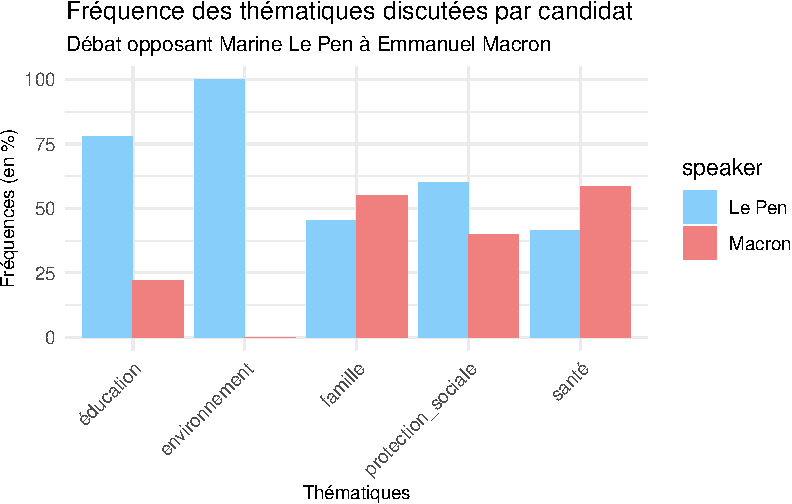
\includegraphics{Travail-Session_files/figure-pdf/unnamed-chunk-2-1.pdf}

}

\end{figure}

\begin{Shaded}
\begin{Highlighting}[]
\NormalTok{Graphique\_2 }\OtherTok{\textless{}{-}} \FunctionTok{ggplot}\NormalTok{(format\_long\_2, }\FunctionTok{aes}\NormalTok{(}\AttributeTok{x =}\NormalTok{ Thématiques, }\AttributeTok{y =}\NormalTok{ Percent, }\AttributeTok{fill =}\NormalTok{ speaker)) }\SpecialCharTok{+} \FunctionTok{geom\_bar}\NormalTok{(}\AttributeTok{stat =}\StringTok{"identity"}\NormalTok{, }\AttributeTok{position =} \StringTok{"dodge"}\NormalTok{) }\SpecialCharTok{+} \FunctionTok{labs}\NormalTok{(}\AttributeTok{title =} \StringTok{"Fréquence des thématiques discutées par candidat"}\NormalTok{, }\AttributeTok{subtitle =} \StringTok{"Débat opposant Ségolène Royal à Nicolas Sarkozy"}\NormalTok{, }\AttributeTok{x =} \StringTok{"Thématiques"}\NormalTok{, }\AttributeTok{y =} \StringTok{"Fréquences (en \%)"}\NormalTok{) }\SpecialCharTok{+} \FunctionTok{scale\_fill\_manual}\NormalTok{ (}\AttributeTok{values =} \FunctionTok{c}\NormalTok{(}\StringTok{"Royal"} \OtherTok{=} \StringTok{"cornflowerblue"}\NormalTok{, }\StringTok{"Sarkozy"} \OtherTok{=} \StringTok{"lightpink1"}\NormalTok{)) }\SpecialCharTok{+} \FunctionTok{theme\_minimal}\NormalTok{() }\SpecialCharTok{+} \FunctionTok{theme}\NormalTok{(}\AttributeTok{axis.text.x.bottom =} \FunctionTok{element\_text}\NormalTok{(}\AttributeTok{angle =} \DecValTok{45}\NormalTok{, }\AttributeTok{hjust =} \DecValTok{1}\NormalTok{), }\AttributeTok{axis.title.x =} \FunctionTok{element\_text}\NormalTok{(}\AttributeTok{size =} \DecValTok{9}\NormalTok{), }\AttributeTok{axis.title.y =} \FunctionTok{element\_text}\NormalTok{(}\AttributeTok{size =} \DecValTok{9}\NormalTok{), }\AttributeTok{plot.title =} \FunctionTok{element\_text}\NormalTok{(}\AttributeTok{size =} \DecValTok{12}\NormalTok{), }\AttributeTok{plot.subtitle =} \FunctionTok{element\_text}\NormalTok{(}\AttributeTok{size =} \DecValTok{10}\NormalTok{))}

\NormalTok{Graphique\_2}
\end{Highlighting}
\end{Shaded}

\begin{figure}[H]

{\centering 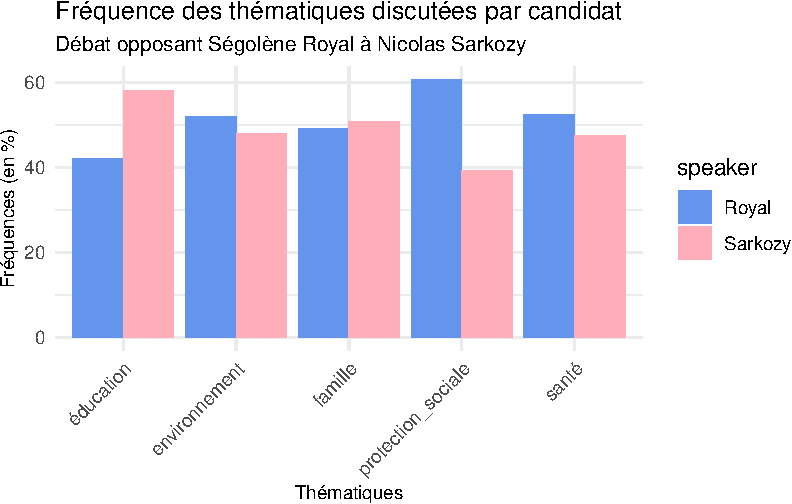
\includegraphics{Travail-Session_files/figure-pdf/unnamed-chunk-2-2.pdf}

}

\end{figure}

\begin{Shaded}
\begin{Highlighting}[]
\NormalTok{Graphique\_3 }\OtherTok{\textless{}{-}} \FunctionTok{ggplot}\NormalTok{(format\_long\_3, }\FunctionTok{aes}\NormalTok{(}\AttributeTok{x =}\NormalTok{ Thématiques, }\AttributeTok{y =}\NormalTok{ Percent, }\AttributeTok{fill =}\NormalTok{ speaker)) }\SpecialCharTok{+} \FunctionTok{geom\_bar}\NormalTok{(}\AttributeTok{stat =} \StringTok{"identity"}\NormalTok{, }\AttributeTok{position =} \StringTok{"dodge"}\NormalTok{) }\SpecialCharTok{+} \FunctionTok{labs}\NormalTok{(}\AttributeTok{title =} \StringTok{"Fréquence des thématiques discutées par candidat"}\NormalTok{, }\AttributeTok{subtitle =} \StringTok{"Débat opposant Jacques Chirac à Lionel Jospin"}\NormalTok{, }\AttributeTok{x =} \StringTok{"Thématiques"}\NormalTok{, }\AttributeTok{y =} \StringTok{"Fréquences (en \%)"}\NormalTok{) }\SpecialCharTok{+} \FunctionTok{scale\_fill\_manual}\NormalTok{(}\AttributeTok{values =} \FunctionTok{c}\NormalTok{(}\StringTok{"Jospin"} \OtherTok{=} \StringTok{"darkgoldenrod1"}\NormalTok{, }\StringTok{"Chirac"} \OtherTok{=} \StringTok{"indianred3"}\NormalTok{)) }\SpecialCharTok{+} \FunctionTok{theme\_minimal}\NormalTok{() }\SpecialCharTok{+} \FunctionTok{theme}\NormalTok{(}\AttributeTok{axis.text.x.bottom =} \FunctionTok{element\_text}\NormalTok{(}\AttributeTok{angle =} \DecValTok{45}\NormalTok{, }\AttributeTok{hjust =} \DecValTok{1}\NormalTok{), }\AttributeTok{axis.title.x =} \FunctionTok{element\_text}\NormalTok{(}\AttributeTok{size =} \DecValTok{9}\NormalTok{), }\AttributeTok{axis.title.y =} \FunctionTok{element\_text}\NormalTok{(}\AttributeTok{size =} \DecValTok{9}\NormalTok{), }\AttributeTok{plot.title =} \FunctionTok{element\_text}\NormalTok{(}\AttributeTok{size =} \DecValTok{12}\NormalTok{), }\AttributeTok{plot.subtitle =} \FunctionTok{element\_text}\NormalTok{(}\AttributeTok{size =} \DecValTok{10}\NormalTok{))}

\NormalTok{Graphique\_3}
\end{Highlighting}
\end{Shaded}

\begin{figure}[H]

{\centering 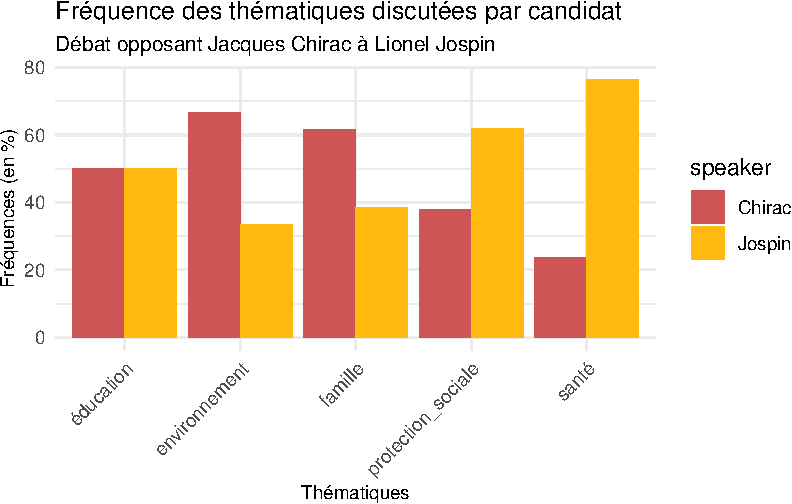
\includegraphics{Travail-Session_files/figure-pdf/unnamed-chunk-2-3.pdf}

}

\end{figure}

\begin{Shaded}
\begin{Highlighting}[]
\NormalTok{Graphique\_4 }\OtherTok{\textless{}{-}} \FunctionTok{ggplot}\NormalTok{(format\_long\_4, }\FunctionTok{aes}\NormalTok{(}\AttributeTok{x =}\NormalTok{ Thématiques, }\AttributeTok{y =}\NormalTok{ Percent, }\AttributeTok{fill =}\NormalTok{ speaker)) }\SpecialCharTok{+} \FunctionTok{geom\_bar}\NormalTok{(}\AttributeTok{stat =} \StringTok{"identity"}\NormalTok{, }\AttributeTok{position =} \StringTok{"dodge"}\NormalTok{) }\SpecialCharTok{+} \FunctionTok{labs}\NormalTok{(}\AttributeTok{title =} \StringTok{"Fréquence des thématiques discutées par candidat"}\NormalTok{, }\AttributeTok{subtitle =} \StringTok{"Débat opposant François Hollande à Nicolas Sarkozy"}\NormalTok{, }\AttributeTok{x =} \StringTok{"Thématiques"}\NormalTok{, }\AttributeTok{y =} \StringTok{"Fréquences (en \%)"}\NormalTok{) }\SpecialCharTok{+} \FunctionTok{scale\_fill\_manual}\NormalTok{(}\AttributeTok{values =} \FunctionTok{c}\NormalTok{(}\StringTok{"Hollande"} \OtherTok{=} \StringTok{"deeppink2"}\NormalTok{, }\StringTok{"Sarkozy"} \OtherTok{=} \StringTok{"cyan3"}\NormalTok{)) }\SpecialCharTok{+} \FunctionTok{theme\_minimal}\NormalTok{() }\SpecialCharTok{+} \FunctionTok{theme}\NormalTok{(}\AttributeTok{axis.text.x.bottom =} \FunctionTok{element\_text}\NormalTok{(}\AttributeTok{angle =} \DecValTok{45}\NormalTok{, }\AttributeTok{hjust =} \DecValTok{1}\NormalTok{), }\AttributeTok{axis.title.x =} \FunctionTok{element\_text}\NormalTok{(}\AttributeTok{size =} \DecValTok{9}\NormalTok{), }\AttributeTok{axis.title.y =} \FunctionTok{element\_text}\NormalTok{(}\AttributeTok{size =} \DecValTok{9}\NormalTok{), }\AttributeTok{plot.title =} \FunctionTok{element\_text}\NormalTok{(}\AttributeTok{size =} \DecValTok{12}\NormalTok{), }\AttributeTok{plot.subtitle =} \FunctionTok{element\_text}\NormalTok{(}\AttributeTok{size =} \DecValTok{10}\NormalTok{))}

\NormalTok{Graphique\_4}
\end{Highlighting}
\end{Shaded}

\begin{figure}[H]

{\centering 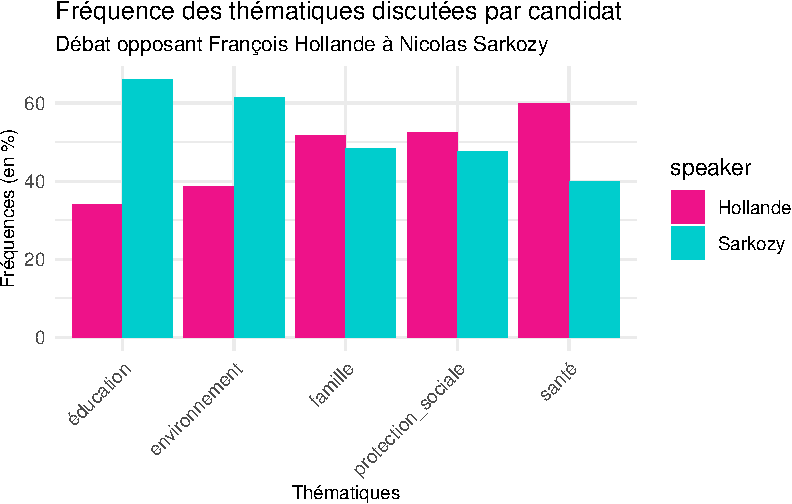
\includegraphics{Travail-Session_files/figure-pdf/unnamed-chunk-2-4.pdf}

}

\end{figure}

\begin{Shaded}
\begin{Highlighting}[]
\CommentTok{\# Graphiques regroupés avec facet\_wrap}

\NormalTok{facet\_graph }\OtherTok{\textless{}{-}} \FunctionTok{ggplot}\NormalTok{(donnees\_finales, }\FunctionTok{aes}\NormalTok{(}\AttributeTok{x =}\NormalTok{ Thématiques, }\AttributeTok{y =}\NormalTok{ Percent, }\AttributeTok{fill =}\NormalTok{ speaker)) }\SpecialCharTok{+} \FunctionTok{geom\_bar}\NormalTok{(}\AttributeTok{stat =} \StringTok{"identity"}\NormalTok{, }\AttributeTok{position =} \StringTok{"dodge"}\NormalTok{) }\SpecialCharTok{+} \FunctionTok{labs}\NormalTok{(}\AttributeTok{title =} \StringTok{"Proportions des thématiques discutées par candidat dans les débats"}\NormalTok{, }\AttributeTok{x =} \StringTok{"Thématiques"}\NormalTok{, }\AttributeTok{y =} \StringTok{"Proportions (en \%)"}\NormalTok{) }\SpecialCharTok{+} \FunctionTok{scale\_fill\_manual}\NormalTok{(}\AttributeTok{values =} \FunctionTok{c}\NormalTok{(}\StringTok{"Le Pen"} \OtherTok{=} \StringTok{"lightskyblue"}\NormalTok{, }\StringTok{"Macron"} \OtherTok{=} \StringTok{"royalblue4"}\NormalTok{, }\StringTok{"Royal"} \OtherTok{=} \StringTok{"mediumpurple2"}\NormalTok{, }\StringTok{"Sarkozy"} \OtherTok{=} \StringTok{"aquamarine3"}\NormalTok{, }\StringTok{"Jospin"} \OtherTok{=} \StringTok{"darkgoldenrod1"}\NormalTok{, }\StringTok{"Chirac"} \OtherTok{=} \StringTok{"indianred3"}\NormalTok{, }\StringTok{"Hollande"} \OtherTok{=} \StringTok{"deeppink2"}\NormalTok{), }\AttributeTok{breaks =} \FunctionTok{c}\NormalTok{(}\StringTok{"Royal"}\NormalTok{, }\StringTok{"Sarkozy"}\NormalTok{, }\StringTok{"Macron"}\NormalTok{, }\StringTok{"Le Pen"}\NormalTok{, }\StringTok{"Jospin"}\NormalTok{, }\StringTok{"Chirac"}\NormalTok{,}\StringTok{"Hollande"}\NormalTok{)) }\SpecialCharTok{+} \FunctionTok{theme\_minimal}\NormalTok{() }\SpecialCharTok{+} \FunctionTok{theme}\NormalTok{(}\AttributeTok{axis.text.x =} \FunctionTok{element\_text}\NormalTok{(}\AttributeTok{angle =} \DecValTok{45}\NormalTok{, }\AttributeTok{hjust =} \DecValTok{1}\NormalTok{), }\AttributeTok{axis.title.x =} \FunctionTok{element\_text}\NormalTok{(}\AttributeTok{size =} \DecValTok{9}\NormalTok{), }\AttributeTok{axis.title.y =} \FunctionTok{element\_text}\NormalTok{(}\AttributeTok{size =} \DecValTok{9}\NormalTok{), }\AttributeTok{plot.title =} \FunctionTok{element\_text}\NormalTok{(}\AttributeTok{size =} \DecValTok{11}\NormalTok{)) }\SpecialCharTok{+} \FunctionTok{facet\_wrap}\NormalTok{(}\SpecialCharTok{\textasciitilde{}}\FunctionTok{factor}\NormalTok{(id, }\AttributeTok{levels =} \FunctionTok{c}\NormalTok{(}\StringTok{"Royal\_Sarkozy"}\NormalTok{, }\StringTok{"Macron\_LePen"}\NormalTok{, }\StringTok{"Jospin\_Chirac"}\NormalTok{, }\StringTok{"Sarkozy\_Hollande"}\NormalTok{)), }\AttributeTok{nrow =} \DecValTok{2}\NormalTok{, }\AttributeTok{scales =} \StringTok{"free\_x"}\NormalTok{)}

\NormalTok{facet\_graph}
\end{Highlighting}
\end{Shaded}

\begin{figure}[H]

{\centering 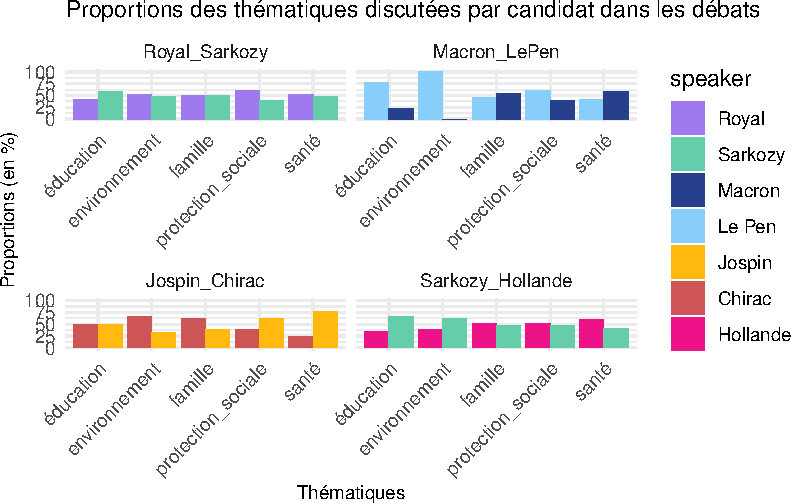
\includegraphics{Travail-Session_files/figure-pdf/unnamed-chunk-2-5.pdf}

}

\end{figure}

\begin{Shaded}
\begin{Highlighting}[]
\CommentTok{\# Comparer les résultats entre les débats généralement}

\NormalTok{donnees\_fin }\OtherTok{\textless{}{-}}\NormalTok{ donnees\_finales }\SpecialCharTok{\%\textgreater{}\%} \FunctionTok{group\_by}\NormalTok{(Thématiques) }\SpecialCharTok{\%\textgreater{}\%} \FunctionTok{mutate}\NormalTok{(}\AttributeTok{somme\_totale =} \FunctionTok{sum}\NormalTok{(Fréquences)) }\SpecialCharTok{\%\textgreater{}\%} \FunctionTok{ungroup}\NormalTok{()}

\NormalTok{donnees\_fin }\OtherTok{\textless{}{-}}\NormalTok{ donnees\_fin }\SpecialCharTok{\%\textgreater{}\%} \FunctionTok{mutate}\NormalTok{(Fréquences}\AttributeTok{\_pourcentage =}\NormalTok{ (Fréquences }\SpecialCharTok{/}\NormalTok{ somme\_totale)}\SpecialCharTok{*}\DecValTok{100}\NormalTok{)}

\NormalTok{donnees\_fin2 }\OtherTok{\textless{}{-}}\NormalTok{ donnees\_fin }\SpecialCharTok{\%\textgreater{}\%} \FunctionTok{group\_by}\NormalTok{(id, Thématiques) }\SpecialCharTok{\%\textgreater{}\%} \FunctionTok{summarize}\NormalTok{(Somme\_Fréquences }\OtherTok{=} \FunctionTok{sum}\NormalTok{(Fréquences\_pourcentage))}
\end{Highlighting}
\end{Shaded}

\begin{verbatim}
`summarise()` has grouped output by 'id'. You can override using the `.groups`
argument.
\end{verbatim}

\begin{Shaded}
\begin{Highlighting}[]
\NormalTok{donnees\_fin2}\SpecialCharTok{$}\NormalTok{id }\OtherTok{\textless{}{-}} \FunctionTok{factor}\NormalTok{(donnees\_fin2}\SpecialCharTok{$}\NormalTok{id, }\AttributeTok{levels =} \FunctionTok{c}\NormalTok{(}\StringTok{"Royal\_Sarkozy"}\NormalTok{, }\StringTok{"Macron\_LePen"}\NormalTok{, }\StringTok{"Jospin\_Chirac"}\NormalTok{, }\StringTok{"Sarkozy\_Hollande"}\NormalTok{))}

\FunctionTok{levels}\NormalTok{(donnees\_fin2}\SpecialCharTok{$}\NormalTok{id)}
\end{Highlighting}
\end{Shaded}

\begin{verbatim}
[1] "Royal_Sarkozy"    "Macron_LePen"     "Jospin_Chirac"    "Sarkozy_Hollande"
\end{verbatim}

\begin{Shaded}
\begin{Highlighting}[]
\NormalTok{Graph\_final\_2 }\OtherTok{\textless{}{-}} \FunctionTok{ggplot}\NormalTok{(donnees\_fin2, }\FunctionTok{aes}\NormalTok{(}\AttributeTok{x =}\NormalTok{ Thématiques , }\AttributeTok{y =}\NormalTok{ Somme\_Fréquences, }\AttributeTok{fill =}\NormalTok{ id)) }\SpecialCharTok{+} \FunctionTok{geom\_bar}\NormalTok{(}\AttributeTok{stat =} \StringTok{"identity"}\NormalTok{, }\AttributeTok{position =} \StringTok{"stack"}\NormalTok{) }\SpecialCharTok{+} \FunctionTok{theme\_minimal}\NormalTok{() }\SpecialCharTok{+} \FunctionTok{labs}\NormalTok{( }\AttributeTok{title =} \StringTok{"Proportions auxquelles les thématiques ont été abordées dans les débats"}\NormalTok{, }\AttributeTok{x =} \StringTok{"Débats électoraux"}\NormalTok{, }\AttributeTok{y =} \StringTok{"Fréquences (en \%)"}\NormalTok{) }\SpecialCharTok{+} \FunctionTok{theme}\NormalTok{(}\AttributeTok{axis.text.x =} \FunctionTok{element\_text}\NormalTok{(}\AttributeTok{angle =} \DecValTok{45}\NormalTok{, }\AttributeTok{hjust =} \DecValTok{1}\NormalTok{, }\AttributeTok{size =} \DecValTok{7}\NormalTok{), }\AttributeTok{axis.title.x =} \FunctionTok{element\_text}\NormalTok{(}\AttributeTok{size =} \DecValTok{9}\NormalTok{), }\AttributeTok{axis.title.y =} \FunctionTok{element\_text}\NormalTok{(}\AttributeTok{size =} \DecValTok{9}\NormalTok{), }\AttributeTok{plot.title =} \FunctionTok{element\_text}\NormalTok{(}\AttributeTok{size =} \DecValTok{12}\NormalTok{)) }\SpecialCharTok{+} \FunctionTok{scale\_fill\_manual}\NormalTok{(}\AttributeTok{values =} \FunctionTok{c}\NormalTok{(}\StringTok{"Jospin\_Chirac"} \OtherTok{=} \StringTok{"lightpink2"}\NormalTok{, }\StringTok{"Macron\_LePen"} \OtherTok{=} \StringTok{"royalblue4"}\NormalTok{, }\StringTok{"Royal\_Sarkozy"} \OtherTok{=} \StringTok{"deepskyblue2"}\NormalTok{, }\StringTok{"Sarkozy\_Hollande"} \OtherTok{=} \StringTok{"deeppink2"}\NormalTok{)) }\SpecialCharTok{+} \FunctionTok{scale\_y\_continuous}\NormalTok{(}\AttributeTok{breaks =} \FunctionTok{c}\NormalTok{(}\DecValTok{0}\NormalTok{, }\DecValTok{10}\NormalTok{, }\DecValTok{20}\NormalTok{, }\DecValTok{30}\NormalTok{, }\DecValTok{40}\NormalTok{, }\DecValTok{50}\NormalTok{, }\DecValTok{60}\NormalTok{, }\DecValTok{70}\NormalTok{, }\DecValTok{80}\NormalTok{, }\DecValTok{90}\NormalTok{, }\DecValTok{100}\NormalTok{))}

\NormalTok{Graph\_final\_2}
\end{Highlighting}
\end{Shaded}

\begin{figure}[H]

{\centering 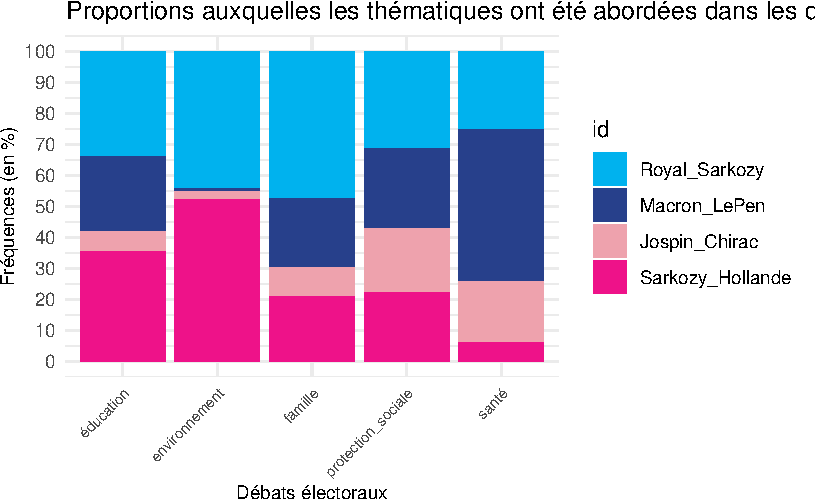
\includegraphics{Travail-Session_files/figure-pdf/unnamed-chunk-2-6.pdf}

}

\end{figure}

\begin{Shaded}
\begin{Highlighting}[]
\CommentTok{\#Contrôler pour le parti politique d\textquotesingle{}appartenance}

\NormalTok{donnees\_fin }\OtherTok{\textless{}{-}}\NormalTok{ donnees\_fin }\SpecialCharTok{\%\textgreater{}\%} \FunctionTok{mutate}\NormalTok{(}\AttributeTok{speaker =} \FunctionTok{ifelse}\NormalTok{(}\FunctionTok{row\_number}\NormalTok{() }\SpecialCharTok{\%in\%} \FunctionTok{c}\NormalTok{(}\DecValTok{26}\SpecialCharTok{:}\DecValTok{30}\NormalTok{), }\StringTok{"Sarkozy2"}\NormalTok{, speaker))}

\NormalTok{donnees\_fin }\OtherTok{\textless{}{-}}\NormalTok{ donnees\_fin }\SpecialCharTok{\%\textgreater{}\%} \FunctionTok{mutate}\NormalTok{(}\AttributeTok{orientation\_partis =} \FunctionTok{case\_when}\NormalTok{(speaker }\SpecialCharTok{==} \StringTok{"Le Pen"}\SpecialCharTok{\textasciitilde{}} \StringTok{"Droite"}\NormalTok{, speaker }\SpecialCharTok{==} \StringTok{"Macron"} \SpecialCharTok{\textasciitilde{}} \StringTok{"Centre"}\NormalTok{, speaker }\SpecialCharTok{==} \StringTok{"Royal"} \SpecialCharTok{\textasciitilde{}} \StringTok{"Gauche"}\NormalTok{, speaker }\SpecialCharTok{==} \StringTok{"Hollande"} \SpecialCharTok{\textasciitilde{}} \StringTok{"Gauche"}\NormalTok{, speaker }\SpecialCharTok{==} \StringTok{"Sarkozy"} \SpecialCharTok{\textasciitilde{}} \StringTok{"Droite"}\NormalTok{, speaker }\SpecialCharTok{==} \StringTok{"Sarkozy2"} \SpecialCharTok{\textasciitilde{}} \StringTok{"Droite"}\NormalTok{, speaker }\SpecialCharTok{==} \StringTok{"Jospin"}\SpecialCharTok{\textasciitilde{}} \StringTok{"Gauche"}\NormalTok{, speaker }\SpecialCharTok{==} \StringTok{"Chirac"} \SpecialCharTok{\textasciitilde{}} \StringTok{"Droite"}\NormalTok{))}

\NormalTok{data\_partis }\OtherTok{\textless{}{-}}\NormalTok{ donnees\_fin }\SpecialCharTok{\%\textgreater{}\%} \FunctionTok{group\_by}\NormalTok{(orientation\_partis, Thématiques) }\SpecialCharTok{\%\textgreater{}\%} \FunctionTok{summarize}\NormalTok{(moyenne\_fréquences }\OtherTok{=} \FunctionTok{mean}\NormalTok{(Fréquences))}
\end{Highlighting}
\end{Shaded}

\begin{verbatim}
`summarise()` has grouped output by 'orientation_partis'. You can override
using the `.groups` argument.
\end{verbatim}

\begin{Shaded}
\begin{Highlighting}[]
\NormalTok{data\_partis }\OtherTok{\textless{}{-}}\NormalTok{ data\_partis[}\SpecialCharTok{{-}}\FunctionTok{c}\NormalTok{(}\DecValTok{1}\NormalTok{, }\DecValTok{2}\NormalTok{, }\DecValTok{3}\NormalTok{, }\DecValTok{4}\NormalTok{, }\DecValTok{5}\NormalTok{), ]}

\NormalTok{Graph\_partis }\OtherTok{\textless{}{-}} \FunctionTok{ggplot}\NormalTok{(data\_partis, }\FunctionTok{aes}\NormalTok{(}\AttributeTok{x =}\NormalTok{ orientation\_partis, }\AttributeTok{y =}\NormalTok{ moyenne\_fréquences, }\AttributeTok{fill =}\NormalTok{ Thématiques)) }\SpecialCharTok{+} \FunctionTok{geom\_bar}\NormalTok{(}\AttributeTok{stat =} \StringTok{"identity"}\NormalTok{, }\AttributeTok{position =} \StringTok{"dodge"}\NormalTok{) }\SpecialCharTok{+} \FunctionTok{labs}\NormalTok{(}\AttributeTok{title =} \StringTok{"Fréquence des thématiques discutées par orientation politique des partis d\textquotesingle{}appartenance"}\NormalTok{, }\AttributeTok{x =} \StringTok{"Orientations politiques"}\NormalTok{, }\AttributeTok{y =} \StringTok{"Fréquences moyennes (en nombre de mots)"}\NormalTok{) }\SpecialCharTok{+} \FunctionTok{scale\_fill\_manual}\NormalTok{(}\AttributeTok{values =} \FunctionTok{c}\NormalTok{(}\StringTok{"environnement"} \OtherTok{=} \StringTok{"forestgreen"}\NormalTok{, }\StringTok{"éducation"} \OtherTok{=} \StringTok{"goldenrod2"}\NormalTok{, }\StringTok{"protection\_sociale"} \OtherTok{=} \StringTok{"deeppink2"}\NormalTok{, }\StringTok{"santé"} \OtherTok{=} \StringTok{"deepskyblue"}\NormalTok{, }\StringTok{"famille"} \OtherTok{=} \StringTok{"royalblue4"}\NormalTok{)) }\SpecialCharTok{+} \FunctionTok{theme\_minimal}\NormalTok{() }\SpecialCharTok{+} \FunctionTok{theme}\NormalTok{(}\AttributeTok{axis.text.x.bottom =} \FunctionTok{element\_text}\NormalTok{(}\AttributeTok{angle =} \DecValTok{45}\NormalTok{, }\AttributeTok{hjust =} \DecValTok{1}\NormalTok{), }\AttributeTok{axis.title.x =} \FunctionTok{element\_text}\NormalTok{(}\AttributeTok{size =} \DecValTok{9}\NormalTok{), }\AttributeTok{axis.title.y =} \FunctionTok{element\_text}\NormalTok{(}\AttributeTok{size =} \DecValTok{9}\NormalTok{), }\AttributeTok{plot.title =} \FunctionTok{element\_text}\NormalTok{(}\AttributeTok{size =} \DecValTok{12}\NormalTok{), }\AttributeTok{plot.subtitle =} \FunctionTok{element\_text}\NormalTok{(}\AttributeTok{size =} \DecValTok{10}\NormalTok{)) }\SpecialCharTok{+} \FunctionTok{scale\_y\_continuous}\NormalTok{(}\AttributeTok{breaks =} \FunctionTok{c}\NormalTok{(}\DecValTok{0}\NormalTok{, }\DecValTok{10}\NormalTok{, }\DecValTok{20}\NormalTok{, }\DecValTok{30}\NormalTok{, }\DecValTok{40}\NormalTok{, }\DecValTok{50}\NormalTok{, }\DecValTok{60}\NormalTok{))}

\NormalTok{Graph\_partis}
\end{Highlighting}
\end{Shaded}

\begin{figure}[H]

{\centering 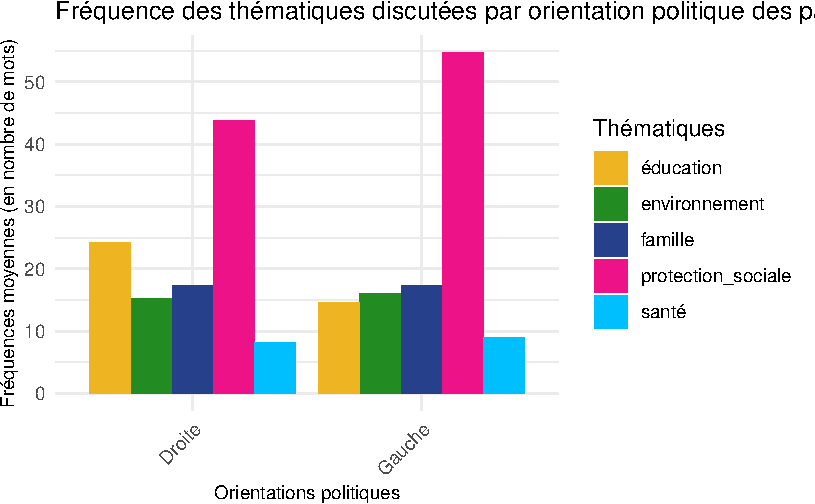
\includegraphics{Travail-Session_files/figure-pdf/unnamed-chunk-2-7.pdf}

}

\end{figure}

\begin{Shaded}
\begin{Highlighting}[]
\NormalTok{candidats\_dg }\OtherTok{\textless{}{-}}\NormalTok{ donnees\_fin }\SpecialCharTok{\%\textgreater{}\%} \FunctionTok{group\_by}\NormalTok{(speaker, orientation\_partis) }\SpecialCharTok{\%\textgreater{}\%} \FunctionTok{summarise}\NormalTok{(Fréquence}\AttributeTok{\_totale =} \FunctionTok{sum}\NormalTok{(Fréquences))}
\end{Highlighting}
\end{Shaded}

\begin{verbatim}
`summarise()` has grouped output by 'speaker'. You can override using the
`.groups` argument.
\end{verbatim}

\begin{Shaded}
\begin{Highlighting}[]
\NormalTok{graph\_orientation\_pol\_candidats }\OtherTok{\textless{}{-}} \FunctionTok{ggplot}\NormalTok{(candidats\_dg, }\FunctionTok{aes}\NormalTok{(}\AttributeTok{x =} \FunctionTok{factor}\NormalTok{(speaker, }\AttributeTok{levels =} \FunctionTok{c}\NormalTok{(}\StringTok{"Chirac"}\NormalTok{, }\StringTok{"Le Pen"}\NormalTok{, }\StringTok{"Sarkozy2"}\NormalTok{, }\StringTok{"Sarkozy"}\NormalTok{,  }\StringTok{"Macron"}\NormalTok{, }\StringTok{"Jospin"}\NormalTok{, }\StringTok{"Hollande"}\NormalTok{, }\StringTok{"Royal"}\NormalTok{)), }\AttributeTok{y =}\NormalTok{ Fréquence\_totale)) }\SpecialCharTok{+} \FunctionTok{geom\_point}\NormalTok{(}\AttributeTok{stat =} \StringTok{"identity"}\NormalTok{, }\AttributeTok{size =} \DecValTok{9}\NormalTok{, }\FunctionTok{aes}\NormalTok{(}\AttributeTok{color =}\NormalTok{ orientation\_partis)) }\SpecialCharTok{+} \FunctionTok{geom\_segment}\NormalTok{(}\FunctionTok{aes}\NormalTok{(}\AttributeTok{x =}\NormalTok{ speaker, }\AttributeTok{xend =}\NormalTok{ speaker, }\AttributeTok{y =} \DecValTok{0}\NormalTok{, }\AttributeTok{yend =}\NormalTok{ Fréquence\_totale, }\AttributeTok{color =}\NormalTok{ orientation\_partis), }\AttributeTok{size =} \DecValTok{3}\NormalTok{) }\SpecialCharTok{+} \FunctionTok{geom\_text}\NormalTok{(}\FunctionTok{aes}\NormalTok{(}\AttributeTok{label =}\NormalTok{ Fréquence\_totale), }\AttributeTok{vjust =} \FloatTok{0.5}\NormalTok{, }\AttributeTok{size =} \DecValTok{3}\NormalTok{, }\AttributeTok{color =} \StringTok{"white"}\NormalTok{) }\SpecialCharTok{+}  \FunctionTok{labs}\NormalTok{(}\AttributeTok{title =} \StringTok{"Fréquences totales des thématiques féminines par candidat"}\NormalTok{, }\AttributeTok{x =} \StringTok{"Candidats"}\NormalTok{, }\AttributeTok{y =} \StringTok{"Fréquences totales"}\NormalTok{) }\SpecialCharTok{+} \FunctionTok{theme\_minimal}\NormalTok{() }\SpecialCharTok{+} \FunctionTok{theme}\NormalTok{(}\AttributeTok{axis.text.x =} \FunctionTok{element\_text}\NormalTok{(}\AttributeTok{angle =} \DecValTok{45}\NormalTok{, }\AttributeTok{hjust =} \DecValTok{1}\NormalTok{), }\AttributeTok{plot.title =} \FunctionTok{element\_text}\NormalTok{(}\AttributeTok{size =} \DecValTok{12}\NormalTok{)) }\SpecialCharTok{+} \FunctionTok{scale\_color\_manual}\NormalTok{(}\AttributeTok{values =} \FunctionTok{c}\NormalTok{(}\StringTok{"Droite"} \OtherTok{=} \StringTok{"royalblue4"}\NormalTok{, }\StringTok{"Centre"} \OtherTok{=} \StringTok{"\#FFB400"}\NormalTok{, }\StringTok{"Gauche"} \OtherTok{=} \StringTok{"firebrick2"}\NormalTok{))}
\end{Highlighting}
\end{Shaded}

\begin{verbatim}
Warning: Using `size` aesthetic for lines was deprecated in ggplot2 3.4.0.
i Please use `linewidth` instead.
\end{verbatim}

\begin{Shaded}
\begin{Highlighting}[]
\NormalTok{graph\_orientation\_pol\_candidats}
\end{Highlighting}
\end{Shaded}

\begin{figure}[H]

{\centering 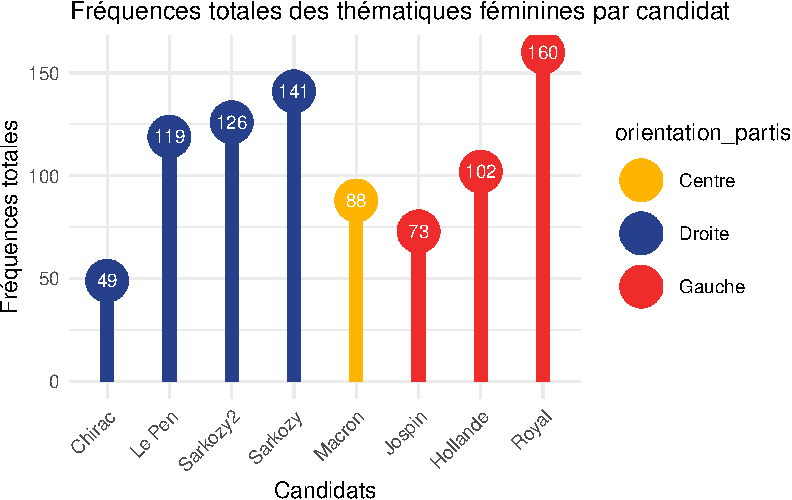
\includegraphics{Travail-Session_files/figure-pdf/unnamed-chunk-2-8.pdf}

}

\end{figure}

\begin{Shaded}
\begin{Highlighting}[]
\NormalTok{graph\_orient\_pol\_2 }\OtherTok{\textless{}{-}} \FunctionTok{ggplot}\NormalTok{(donnees\_fin, }\FunctionTok{aes}\NormalTok{(}\AttributeTok{x =} \FunctionTok{factor}\NormalTok{(speaker, }\AttributeTok{levels =} \FunctionTok{c}\NormalTok{(}\StringTok{"Chirac"}\NormalTok{, }\StringTok{"Sarkozy"}\NormalTok{,}\StringTok{"Sarkozy2"}\NormalTok{, }\StringTok{"Le Pen"}\NormalTok{, }\StringTok{"Macron"}\NormalTok{, }\StringTok{"Jospin"}\NormalTok{, }\StringTok{"Royal"}\NormalTok{, }\StringTok{"Hollande"}\NormalTok{)), }\AttributeTok{y =}\NormalTok{ Fréquences\_pourcentage)) }\SpecialCharTok{+} \FunctionTok{geom\_bar}\NormalTok{(}\AttributeTok{stat =} \StringTok{"identity"}\NormalTok{,}\AttributeTok{position =} \StringTok{"dodge"}\NormalTok{, }\FunctionTok{aes}\NormalTok{(}\AttributeTok{fill =}\NormalTok{ orientation\_partis)) }\SpecialCharTok{+} \FunctionTok{labs}\NormalTok{(}\AttributeTok{title =} \StringTok{"Proportions des thématiques féminines relevées dans le discours des candidats"}\NormalTok{, }\AttributeTok{x =} \StringTok{"Candidats"}\NormalTok{, }\AttributeTok{y =} \StringTok{"Proportions (en \%)"}\NormalTok{) }\SpecialCharTok{+} \FunctionTok{theme\_minimal}\NormalTok{() }\SpecialCharTok{+} \FunctionTok{theme}\NormalTok{(}\AttributeTok{axis.text.x =} \FunctionTok{element\_text}\NormalTok{(}\AttributeTok{angle =} \DecValTok{45}\NormalTok{, }\AttributeTok{hjust =} \DecValTok{1}\NormalTok{), }\AttributeTok{plot.title =} \FunctionTok{element\_text}\NormalTok{(}\AttributeTok{size =} \DecValTok{11}\NormalTok{)) }\SpecialCharTok{+} \FunctionTok{scale\_fill\_manual}\NormalTok{(}\AttributeTok{values =} \FunctionTok{c}\NormalTok{(}\StringTok{"Droite"} \OtherTok{=} \StringTok{"royalblue4"}\NormalTok{, }\StringTok{"Centre"} \OtherTok{=} \StringTok{"\#FFB400"}\NormalTok{, }\StringTok{"Gauche"} \OtherTok{=} \StringTok{"firebrick2"}\NormalTok{)) }\SpecialCharTok{+} \FunctionTok{facet\_wrap}\NormalTok{(}\SpecialCharTok{\textasciitilde{}}\NormalTok{ Thématiques, }\AttributeTok{scales =} \StringTok{"free\_x"}\NormalTok{)}

\NormalTok{graph\_orient\_pol\_2}
\end{Highlighting}
\end{Shaded}

\begin{figure}[H]

{\centering 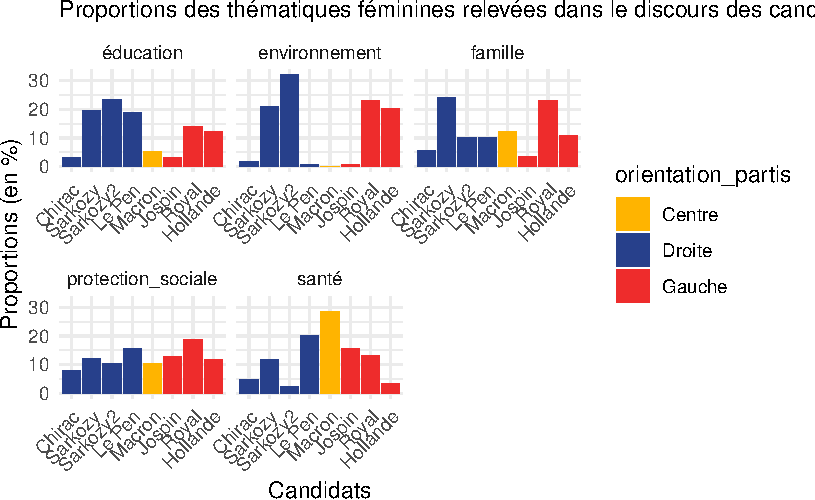
\includegraphics{Travail-Session_files/figure-pdf/unnamed-chunk-2-9.pdf}

}

\end{figure}

\begin{Shaded}
\begin{Highlighting}[]
\CommentTok{\# Contrôler pour le contexte}

\NormalTok{contexte }\OtherTok{\textless{}{-}}\NormalTok{ donnees\_fin }\SpecialCharTok{\%\textgreater{}\%} \FunctionTok{group\_by}\NormalTok{(id, Thématiques) }\SpecialCharTok{\%\textgreater{}\%} \FunctionTok{summarise}\NormalTok{(Fréquences}\AttributeTok{\_totales =} \FunctionTok{sum}\NormalTok{(Fréquences)) }\SpecialCharTok{\%\textgreater{}\%} \FunctionTok{ungroup}\NormalTok{()}
\end{Highlighting}
\end{Shaded}

\begin{verbatim}
`summarise()` has grouped output by 'id'. You can override using the `.groups`
argument.
\end{verbatim}

\begin{Shaded}
\begin{Highlighting}[]
\NormalTok{contexte }\OtherTok{\textless{}{-}}\NormalTok{ contexte }\SpecialCharTok{\%\textgreater{}\%} \FunctionTok{mutate}\NormalTok{(}\AttributeTok{year =} \FunctionTok{case\_when}\NormalTok{(id }\SpecialCharTok{==} \StringTok{"Royal\_Sarkozy"}\SpecialCharTok{\textasciitilde{}}\StringTok{"2007"}\NormalTok{, id }\SpecialCharTok{==} \StringTok{"Macron\_LePen"} \SpecialCharTok{\textasciitilde{}} \StringTok{"2017"}\NormalTok{, id }\SpecialCharTok{==} \StringTok{"Sarkozy\_Hollande"} \SpecialCharTok{\textasciitilde{}} \StringTok{"2012"}\NormalTok{, id }\SpecialCharTok{==} \StringTok{"Jospin\_Chirac"} \SpecialCharTok{\textasciitilde{}} \StringTok{"1995"}\NormalTok{))}

\NormalTok{contexte }\OtherTok{\textless{}{-}} \FunctionTok{pivot\_wider}\NormalTok{(contexte, }\AttributeTok{id\_cols =} \FunctionTok{c}\NormalTok{(id, year), }\AttributeTok{names\_from =}\NormalTok{ Thématiques, }\AttributeTok{values\_from =}\NormalTok{ Fréquences\_totales)}

\NormalTok{contexte }\OtherTok{\textless{}{-}}\NormalTok{ tidyr}\SpecialCharTok{::}\FunctionTok{pivot\_longer}\NormalTok{(contexte, }\AttributeTok{cols =} \FunctionTok{c}\NormalTok{(environnement, famille, protection\_sociale, santé, éducation), }\AttributeTok{names\_to =} \StringTok{"Thématiques"}\NormalTok{, }\AttributeTok{values\_to =} \StringTok{"Fréquences"}\NormalTok{)}
 
\NormalTok{contexte }\OtherTok{\textless{}{-}}\NormalTok{ contexte }\SpecialCharTok{\%\textgreater{}\%} \FunctionTok{group\_by}\NormalTok{(Thématiques) }\SpecialCharTok{\%\textgreater{}\%} \FunctionTok{mutate}\NormalTok{(}\AttributeTok{Percent =}\NormalTok{ Fréquences }\SpecialCharTok{/} \FunctionTok{sum}\NormalTok{(Fréquences) }\SpecialCharTok{*} \DecValTok{100}\NormalTok{)}
 
\NormalTok{graph\_contexte }\OtherTok{\textless{}{-}} \FunctionTok{ggplot}\NormalTok{(contexte, }\FunctionTok{aes}\NormalTok{(}\AttributeTok{x =}\NormalTok{ year, }\AttributeTok{y =}\NormalTok{ Percent, }\AttributeTok{group =}\NormalTok{ Thématiques, }\AttributeTok{color =}\NormalTok{ Thématiques)) }\SpecialCharTok{+} \FunctionTok{geom\_line}\NormalTok{() }\SpecialCharTok{+} \FunctionTok{geom\_point}\NormalTok{() }\SpecialCharTok{+} \FunctionTok{labs}\NormalTok{(}\AttributeTok{title =} \StringTok{"Évolution de la saillance des thématiques féminines au fil des débats de 1995 à 2017"}\NormalTok{, }\AttributeTok{x =} \StringTok{"Années"}\NormalTok{, }\AttributeTok{y =} \StringTok{"Proportions de mots relevés (en \%)"}\NormalTok{) }\SpecialCharTok{+} \FunctionTok{theme\_minimal}\NormalTok{() }\SpecialCharTok{+} \FunctionTok{scale\_color\_manual}\NormalTok{(}\AttributeTok{values =} \FunctionTok{c}\NormalTok{(}\StringTok{"environnement"} \OtherTok{=} \StringTok{"forestgreen"}\NormalTok{, }\StringTok{"santé"} \OtherTok{=} \StringTok{"deepskyblue"}\NormalTok{, }\StringTok{"éducation"} \OtherTok{=} \StringTok{"goldenrod2"}\NormalTok{, }\StringTok{"protection\_sociale"} \OtherTok{=} \StringTok{"deeppink2"}\NormalTok{, }\StringTok{"famille"} \OtherTok{=} \StringTok{"royalblue4"}\NormalTok{)) }\SpecialCharTok{+} \FunctionTok{theme}\NormalTok{(}\AttributeTok{plot.title =} \FunctionTok{element\_text}\NormalTok{(}\AttributeTok{size =} \DecValTok{10}\NormalTok{))}

\NormalTok{ graph\_contexte}
\end{Highlighting}
\end{Shaded}

\begin{figure}[H]

{\centering 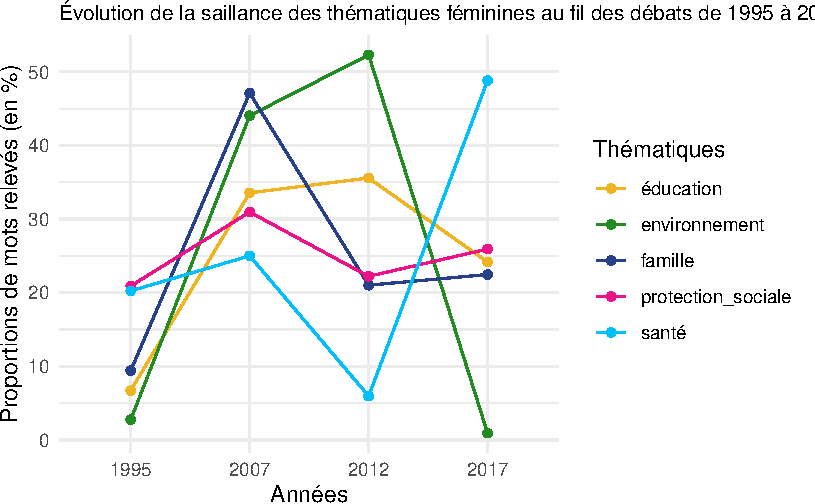
\includegraphics{Travail-Session_files/figure-pdf/unnamed-chunk-2-10.pdf}

}

\end{figure}



\end{document}
